% Created 2023-04-06 Thu 14:18
% Intended LaTeX compiler: pdflatex
\documentclass[14pt]{extarticle}
\usepackage[utf8]{inputenc}
\usepackage[T2A]{fontenc}
\usepackage{graphicx}
\usepackage{longtable}
\usepackage{wrapfig}
\usepackage{rotating}
\usepackage[normalem]{ulem}
\usepackage{amsmath}
\usepackage{amssymb}
\usepackage{capt-of}
\usepackage{hyperref}
\usepackage[russian]{babel}
\usepackage{tempora}
\usepackage{geometry}
\geometry{a4paper, left=30mm, top=20mm, bottom=20mm, right=15mm }
\usepackage{graphicx}
\usepackage{array}
\usepackage{tabularx}
\usepackage{listings}
\usepackage{float}
\usepackage{setspace}
\usepackage{tabularx}
\usepackage{longtable}
\usepackage{titlesec}
\titleformat*{\section}{\large\bfseries}
\titleformat*{\subsection}{\normalsize\bfseries}
\titleformat*{\subsubsection}{\normalsize\bfseries}
\addto\captionsrussian{\renewcommand{\contentsname}{\centering \normalsize СОДЕРЖАНИЕ}}
\addtocontents{toc}{\protect\thispagestyle{empty}}
\usepackage{titletoc}
\titlecontents{section}[0pt]{}{\contentsmargin{0pt} \thecontentslabel\enspace}{\contentsmargin{0pt}}{\titlerule*[0.5pc]{.}\contentspage}[]
\dottedcontents{subsection}[3.1em]{}{1.5em}{0.5pc}
\usepackage{caption}
\DeclareCaptionLabelSeparator{custom}{ -- }
\captionsetup[figure]{name=Рисунок, labelsep=custom, font={onehalfspacing}, justification=centering}
\usepackage{ragged2e}
\justifying
\setlength\parindent{1.25cm}
\sloppy
\usepackage{indentfirst}
\usepackage{multirow}
\usepackage{lscape}
\author{Панков Вася}
\date{\today}
\title{МДК 02.02 Инструментальные средства разработки}
\hypersetup{
 pdfauthor={Панков Вася},
 pdftitle={МДК 02.02 Инструментальные средства разработки},
 pdfkeywords={},
 pdfsubject={Опалева У.С.},
 pdfcreator={Emacs 30.0.50 (Org mode 9.6.2)}, 
 pdflang={Russian}}

% Setup for code blocks [1/2]

\usepackage{fvextra}

\fvset{%
  commandchars=\\\{\},
  highlightcolor=white!95!black!80!blue,
  breaklines=true,
  breaksymbol=\color{white!60!black}\tiny\ensuremath{\hookrightarrow}}

% Make line numbers smaller and grey.
\renewcommand\theFancyVerbLine{\footnotesize\color{black!40!white}\arabic{FancyVerbLine}}

\usepackage{xcolor}

% In case engrave-faces-latex-gen-preamble has not been run.
\providecolor{EfD}{HTML}{f7f7f7}
\providecolor{EFD}{HTML}{28292e}

% Define a Code environment to prettily wrap the fontified code.
\usepackage[breakable,xparse]{tcolorbox}
\DeclareTColorBox[]{Code}{o}%
{colback=EfD!98!EFD, colframe=EfD!95!EFD,
  fontupper=\footnotesize\setlength{\fboxsep}{0pt},
  colupper=EFD,
  IfNoValueTF={#1}%
  {boxsep=2pt, arc=2.5pt, outer arc=2.5pt,
    boxrule=0.5pt, left=2pt}%
  {boxsep=2.5pt, arc=0pt, outer arc=0pt,
    boxrule=0pt, leftrule=1.5pt, left=0.5pt},
  right=2pt, top=1pt, bottom=0.5pt,
  breakable}

% Support listings with captions
\usepackage{float}
\floatstyle{plain}
\newfloat{listing}{htbp}{lst}
\newcommand{\listingsname}{Listing}
\floatname{listing}{\listingsname}
\newcommand{\listoflistingsname}{List of Listings}
\providecommand{\listoflistings}{\listof{listing}{\listoflistingsname}}


% Setup for code blocks [2/2]: syntax highlighting colors

\newcommand\efstrut{\vrule height 2.1ex depth 0.8ex width 0pt}
\definecolor{EFD}{HTML}{212121}
\definecolor{EfD}{HTML}{FAFAFA}
\newcommand{\EFD}[1]{\textcolor{EFD}{#1}} % default
\definecolor{EFh}{HTML}{607d8b}
\newcommand{\EFh}[1]{\textcolor{EFh}{#1}} % shadow
\definecolor{EFsc}{HTML}{4eee94}
\newcommand{\EFsc}[1]{\textcolor{EFsc}{#1}} % success
\definecolor{EFw}{HTML}{FF5722}
\newcommand{\EFw}[1]{\textcolor{EFw}{#1}} % warning
\definecolor{EFe}{HTML}{B71C1C}
\newcommand{\EFe}[1]{\textcolor{EFe}{#1}} % error
\definecolor{EFc}{HTML}{607d8b}
\newcommand{\EFc}[1]{\textcolor{EFc}{#1}} % font-lock-comment-face
\definecolor{EFcd}{HTML}{607d8b}
\newcommand{\EFcd}[1]{\textcolor{EFcd}{#1}} % font-lock-comment-delimiter-face
\definecolor{EFs}{HTML}{689f38}
\newcommand{\EFs}[1]{\textcolor{EFs}{#1}} % font-lock-string-face
\definecolor{EFd}{HTML}{673ab7}
\newcommand{\EFd}[1]{\textcolor{EFd}{#1}} % font-lock-doc-face
\definecolor{EFm}{HTML}{558b2f}
\newcommand{\EFm}[1]{\textcolor{EFm}{#1}} % font-lock-doc-markup-face
\definecolor{EFk}{HTML}{00796b}
\newcommand{\EFk}[1]{\textcolor{EFk}{#1}} % font-lock-keyword-face
\definecolor{EFb}{HTML}{B71C1C}
\newcommand{\EFb}[1]{\textcolor{EFb}{#1}} % font-lock-builtin-face
\definecolor{EFf}{HTML}{0097A7}
\newcommand{\EFf}[1]{\textcolor{EFf}{#1}} % font-lock-function-name-face
\definecolor{EFv}{HTML}{EF6C00}
\newcommand{\EFv}[1]{\textcolor{EFv}{#1}} % font-lock-variable-name-face
\definecolor{EFt}{HTML}{0097A7}
\newcommand{\EFt}[1]{\textcolor{EFt}{#1}} % font-lock-type-face
\definecolor{EFo}{HTML}{558b2f}
\newcommand{\EFo}[1]{\textcolor{EFo}{#1}} % font-lock-constant-face
\definecolor{EFwr}{HTML}{B71C1C}
\newcommand{\EFwr}[1]{\textcolor{EFwr}{\textbf{#1}}} % font-lock-warning-face
\definecolor{EFnc}{HTML}{2196f3}
\newcommand{\EFnc}[1]{\textcolor{EFnc}{#1}} % font-lock-negation-char-face
\definecolor{EFpp}{HTML}{FFA000}
\newcommand{\EFpp}[1]{\textcolor{EFpp}{#1}} % font-lock-preprocessor-face
\definecolor{EFrc}{HTML}{4527A0}
\newcommand{\EFrc}[1]{\textcolor{EFrc}{#1}} % font-lock-regexp-grouping-construct
\definecolor{EFrb}{HTML}{FFA000}
\newcommand{\EFrb}[1]{\textcolor{EFrb}{#1}} % font-lock-regexp-grouping-backslash
\definecolor{Efob}{HTML}{EFEBE9}
\newcommand{\EFob}[1]{\colorbox{Efob}{\efstrut{}#1}} % org-block
\newcommand{\EFhn}[1]{#1} % highlight-numbers-number
\newcommand{\EFhq}[1]{#1} % highlight-quoted-quote
\newcommand{\EFhs}[1]{#1} % highlight-quoted-symbol
\newcommand{\EFrda}[1]{#1} % rainbow-delimiters-depth-1-face
\newcommand{\EFrdb}[1]{#1} % rainbow-delimiters-depth-2-face
\newcommand{\EFrdc}[1]{#1} % rainbow-delimiters-depth-3-face
\newcommand{\EFrdd}[1]{#1} % rainbow-delimiters-depth-4-face
\newcommand{\EFrde}[1]{#1} % rainbow-delimiters-depth-5-face
\newcommand{\EFrdf}[1]{#1} % rainbow-delimiters-depth-6-face
\newcommand{\EFrdg}[1]{#1} % rainbow-delimiters-depth-7-face
\newcommand{\EFrdh}[1]{#1} % rainbow-delimiters-depth-8-face
\newcommand{\EFrdi}[1]{#1} % rainbow-delimiters-depth-9-face
\begin{document}

\begin{titlepage}

\centering{ГУАП}

\vspace{32pt}

\centering{ФАКУЛЬТЕТ СРЕДНЕГО ПРОФЕССИОНАЛЬНОГО ОБРАЗОВАНИЯ}

\vspace{60pt}

\raggedright{ОТЧЕТ \\
ЗАЩИЩЕН С ОЦЕНКОЙ}
\vspace{14pt}

\raggedright{ПРЕПОДАВАТЕЛЬ}

\vspace{12pt}

\begin{tabularx}{\textwidth}{ >{\centering\arraybackslash}X >{\centering\arraybackslash}X >{\centering\arraybackslash}X }
	 преподаватель & & Опалева У.С. \\ 
	 \hrulefill & \hrulefill & \hrulefill \\ 
\footnotesize{должность, уч. степень, звание} & \footnotesize{подпись, дата} & \footnotesize{инициалы, фамилия} \\ 
\end{tabularx} 
 
\vspace{48pt} 

\centering{ОТЧЕТЫ О ЛАБОРАТОРНЫХ РАБОТАХ} 

\vspace{76pt} 

\centering{По дисциплине: МДК 02.02 Инструментальные средства разработки} 

\vspace*{\fill} 

\raggedright{РАБОТУ ВЫПОЛНИЛ} 

\vspace{10pt} 

\begin{tabularx}{\textwidth}{>{\raggedright\arraybackslash}X  >{\centering\arraybackslash}X >{\centering\arraybackslash}X >{\centering\arraybackslash}X }
	 СТУДЕНТ ГР. № & 021к & & Панков Вася \\ 
	 & \hrulefill & \hrulefill & \hrulefill \\ 
	 &  & \footnotesize{подпись, дата} & \footnotesize{инициалы, фамилия} \\ 
\end{tabularx} 
 
\vspace*{\fill} 

\centering{Санкт-Петербург \the\year} 

\end{titlepage}

\tableofcontents \clearpage

\section{Лабораторная работа №2-4}
\label{sec:orgc0008a6}

Тема: Разработка структуры проекта. Диаграмма модулей. Перечень артефактов и протоколов. Настройка работы системы контроля версий. Разработка проекта на основании шаблона. 

Цель: создание модульной структуры проекта в виде диаграммы, разработка перечня артефактов (основных файлов) и протоколов, настройка Git 


Выполнение работы:

​1. Требуется создать веб-приложение (сайт) на основе имеющегося шаблона. Выбрать Файл > Создать > Проект (Create a new project). Далее в открывшемся окне выбрать Bottle Web Project и нажать Next: 

Задать название проекта (в наименование должна быть включена фамилия студента) > Create.

\begin{figure}[H]
\centering
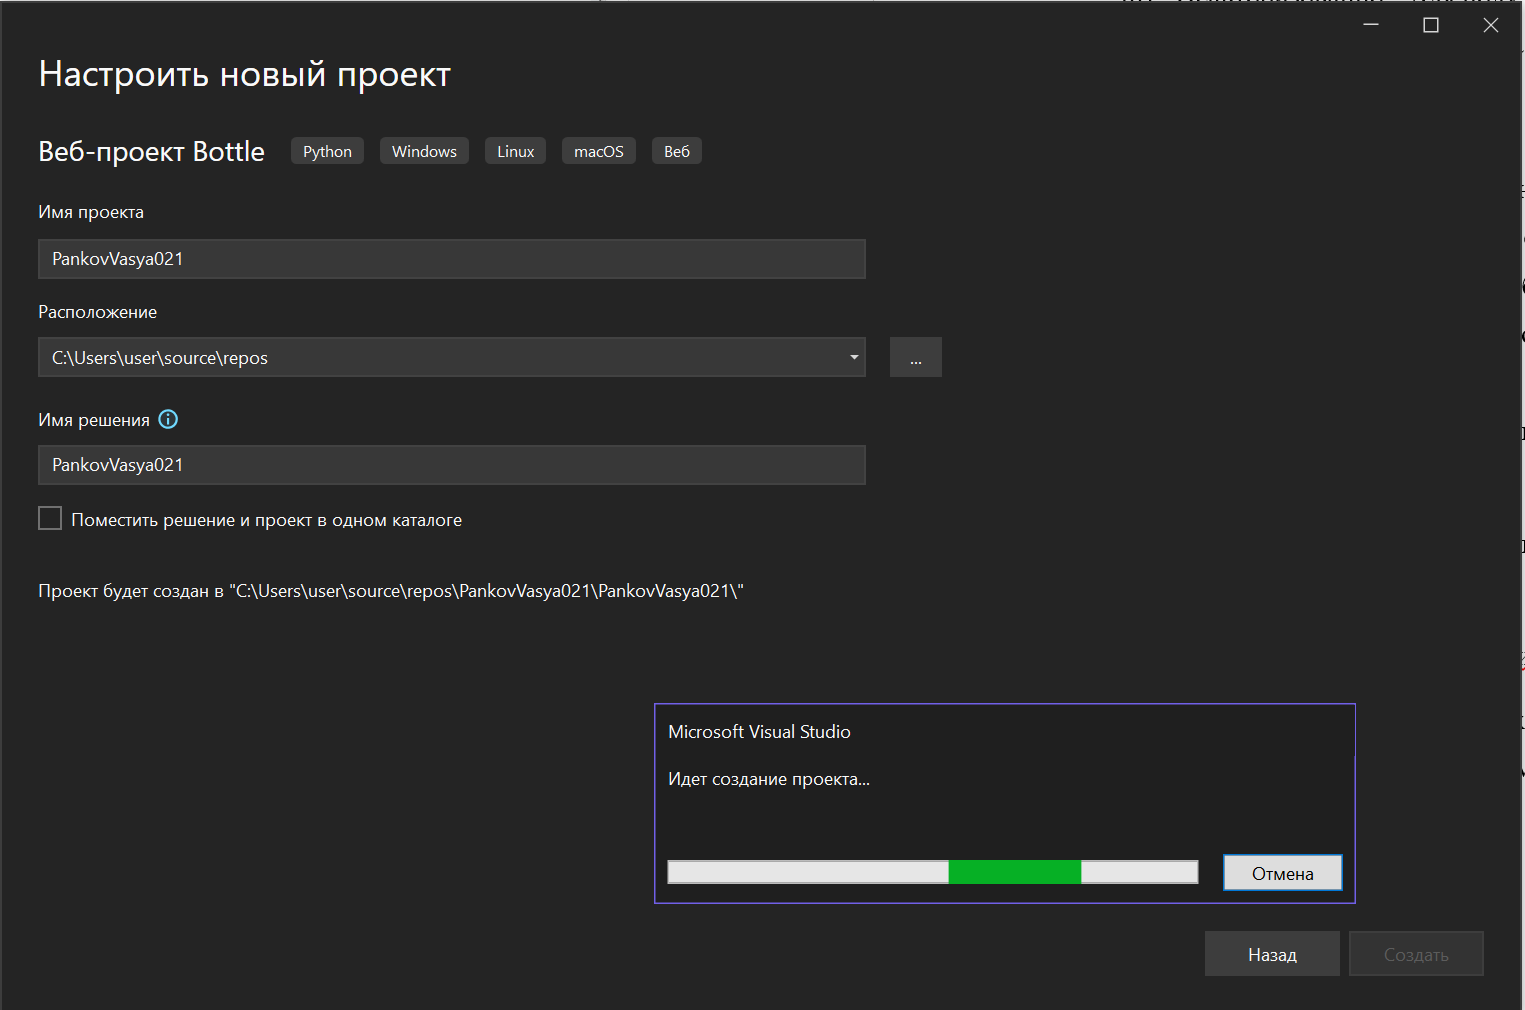
\includegraphics[width=.9\linewidth]{images/20230323-120448_screenshot.png}
\caption{Создание решения}
\end{figure}


​2. По умолчанию в редакторе кода откроется файл app.py. Для корректной интерпретации содержимого файла requirements.txt будет предложено создать виртуальное окружение.

\begin{figure}[H]
\centering
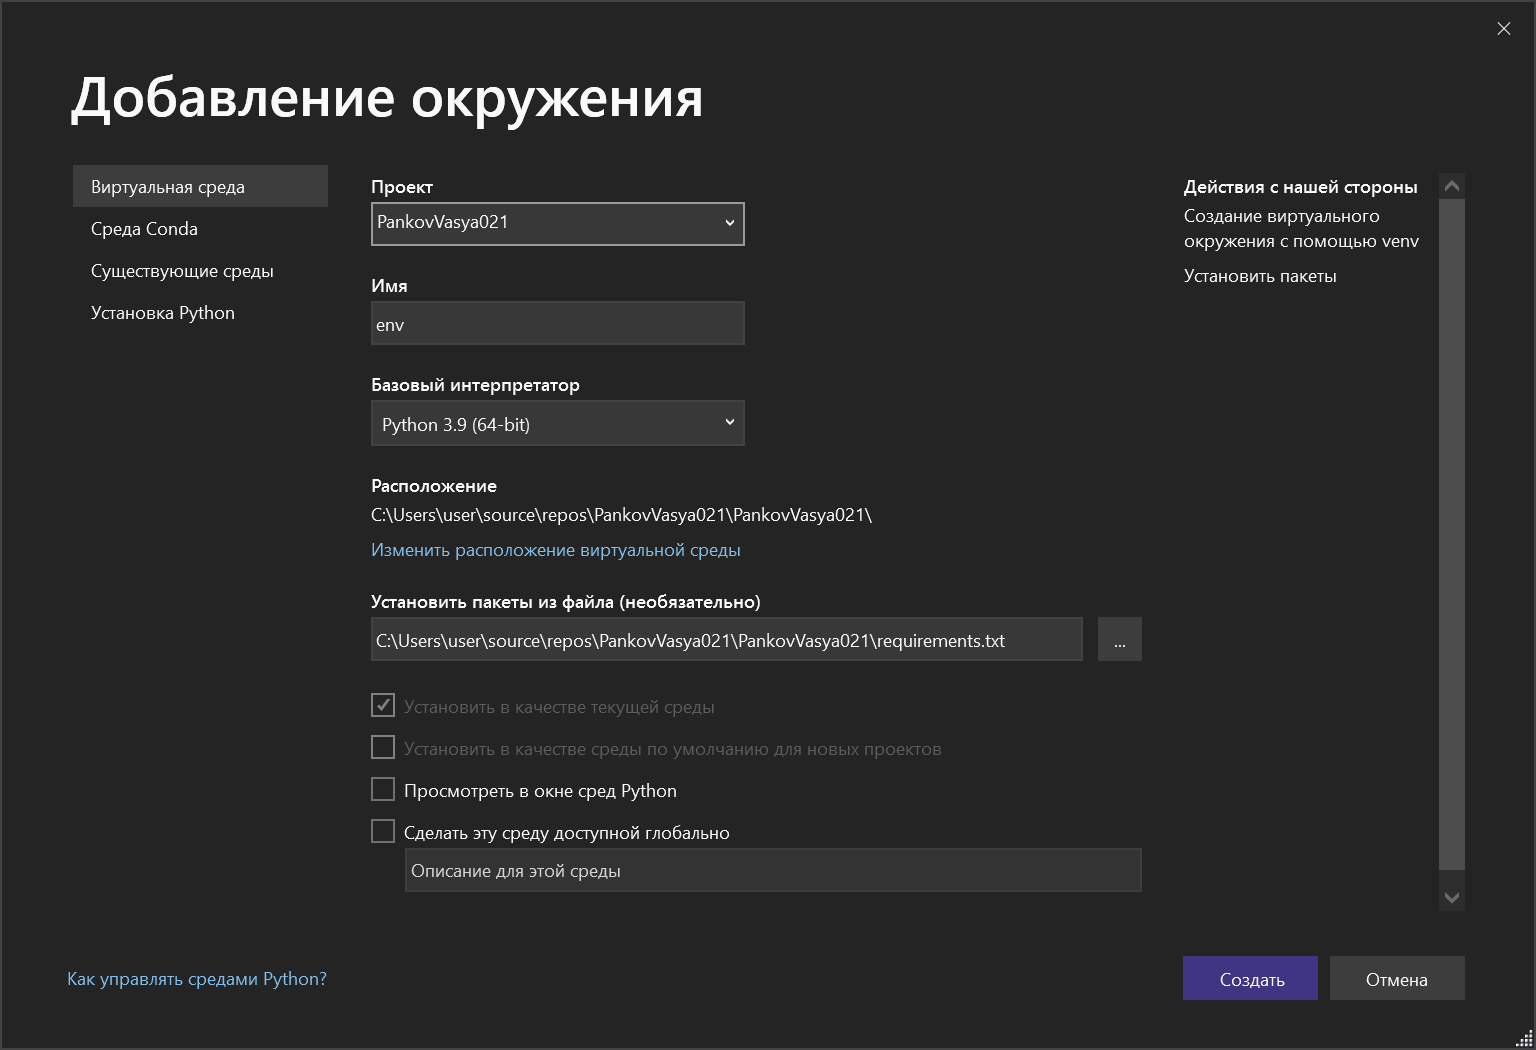
\includegraphics[width=.9\linewidth]{images/20230323-120529_screenshot.png}
\caption{Создание виртуальной среды}
\end{figure}

\begin{figure}[H]
\centering
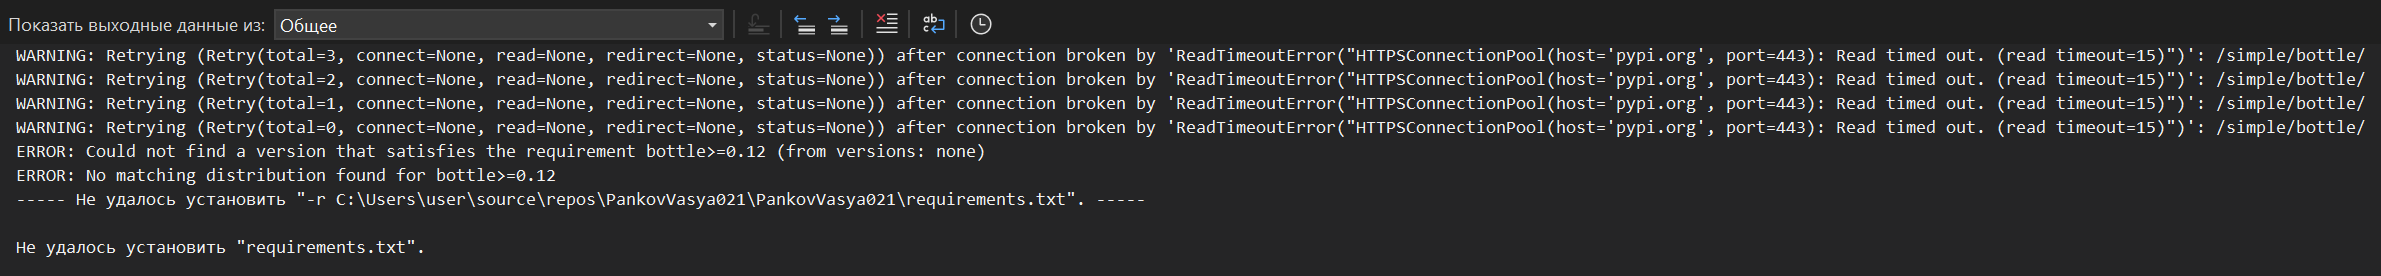
\includegraphics[width=.9\linewidth]{images/20230323-121117_screenshot.png}
\caption{Неудачная разработка среды}
\end{figure}



​3. Ознакомиться со структурой проекта, открыв Обозреватель решений (Solution Explorer): 

В папке static содержатся стилевые css-файлы для оформления внешнего вида веб-страниц, шрифтовые наборы и js-скрипты. 

Выбрав для просмотра файлы из папки views, можно убедиться, что они представляют собой макеты веб-страниц: главной (index.tpl), о нас (about.tpl), контакты (contact.tpl),
а файл layout.tpl – не что иное, как шаблон обёртки с панелью навигации, содержащей четыре гиперссылки: Application name, Home, About, Contact в «шапке» сайта и небольшим «подвалом».

\begin{figure}[H]
\centering
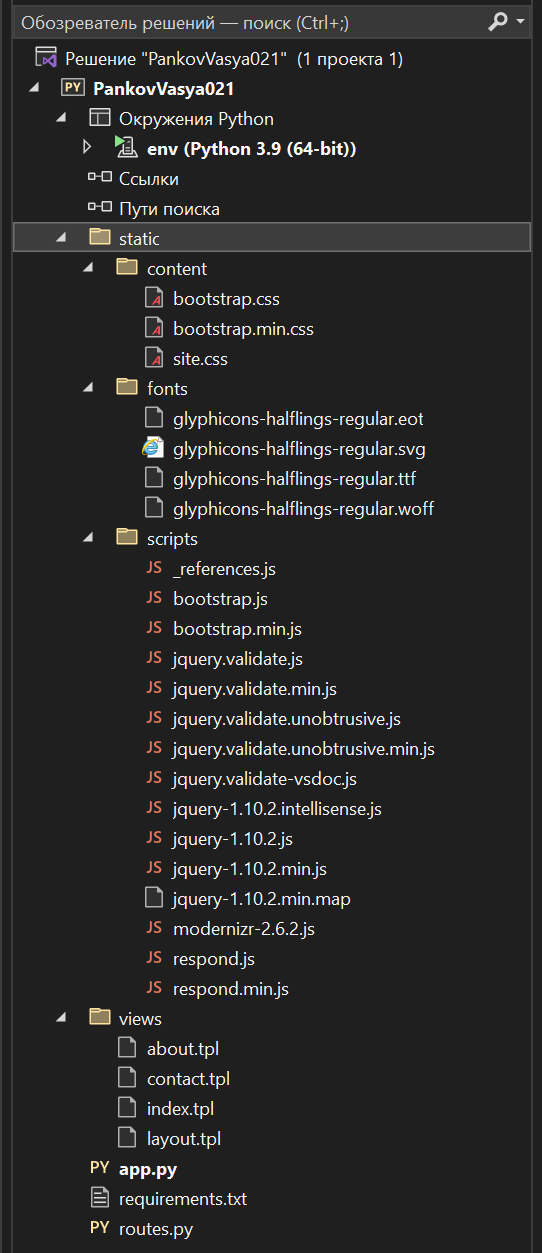
\includegraphics[height=10cm]{images/20230323-120758_screenshot.png}
\caption{Структура проекта}
\end{figure}

\begin{figure}[H]
\centering

\includegraphics[width=.9\linewidth]{images/20230323-121247_screenshot.png}
\caption{Удачная установка}
\end{figure}


​4. Выполнить запуск проекта

\begin{figure}[H]
\centering
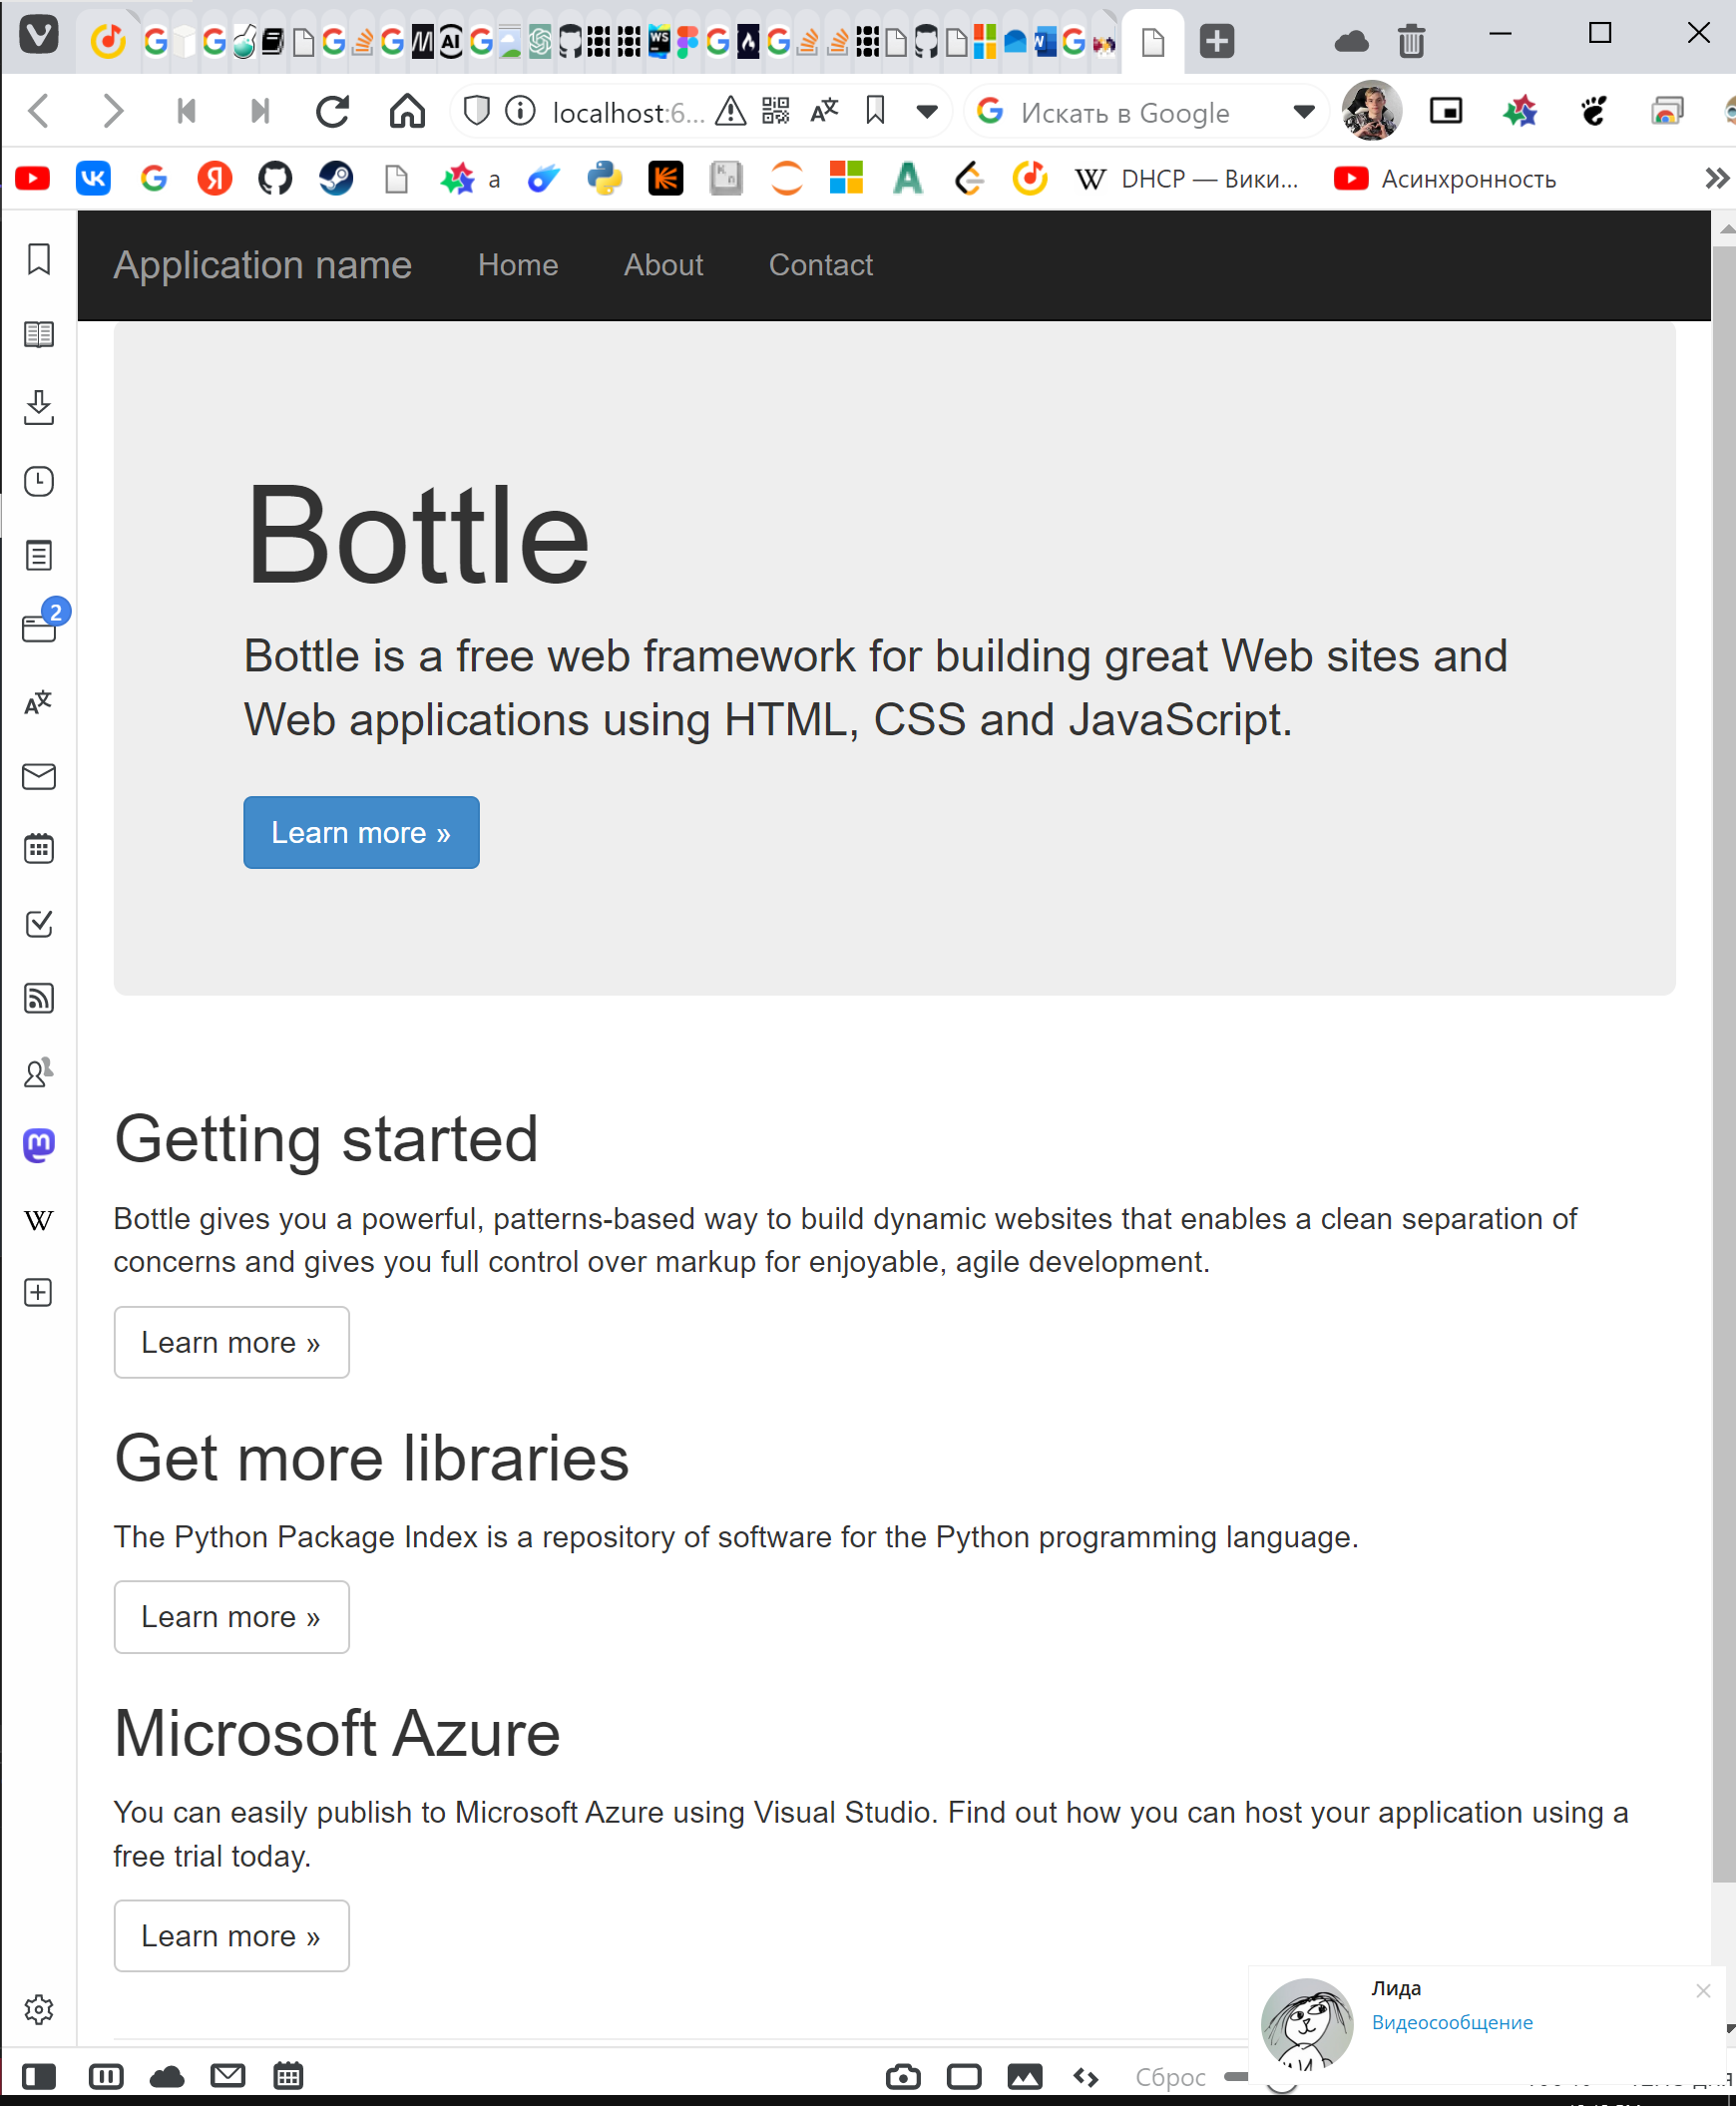
\includegraphics[width=.9\linewidth]{images/20230323-121321_screenshot.png}
\caption{Запуск проекта}
\end{figure}


​​​5. Например, вместо текста заголовка «Bottle» на главной (домашней) странице требуется разместить картинку.
   Для этого сначала в структуре каталога static создаётся папка images, в которую копируется файл изображения logo\textsubscript{nav.png}.
   Затем в коде index.tpl удалить строку <h1> Bottle </h1>, добавить <img src="static\images\logo\textsubscript{nav.png}">
   (файл изображения можно скачать с сайта \url{http://bottlepy.org/docs/dev/index.html}) и пустой абзац <p> </p>

\begin{figure}[H]
\centering
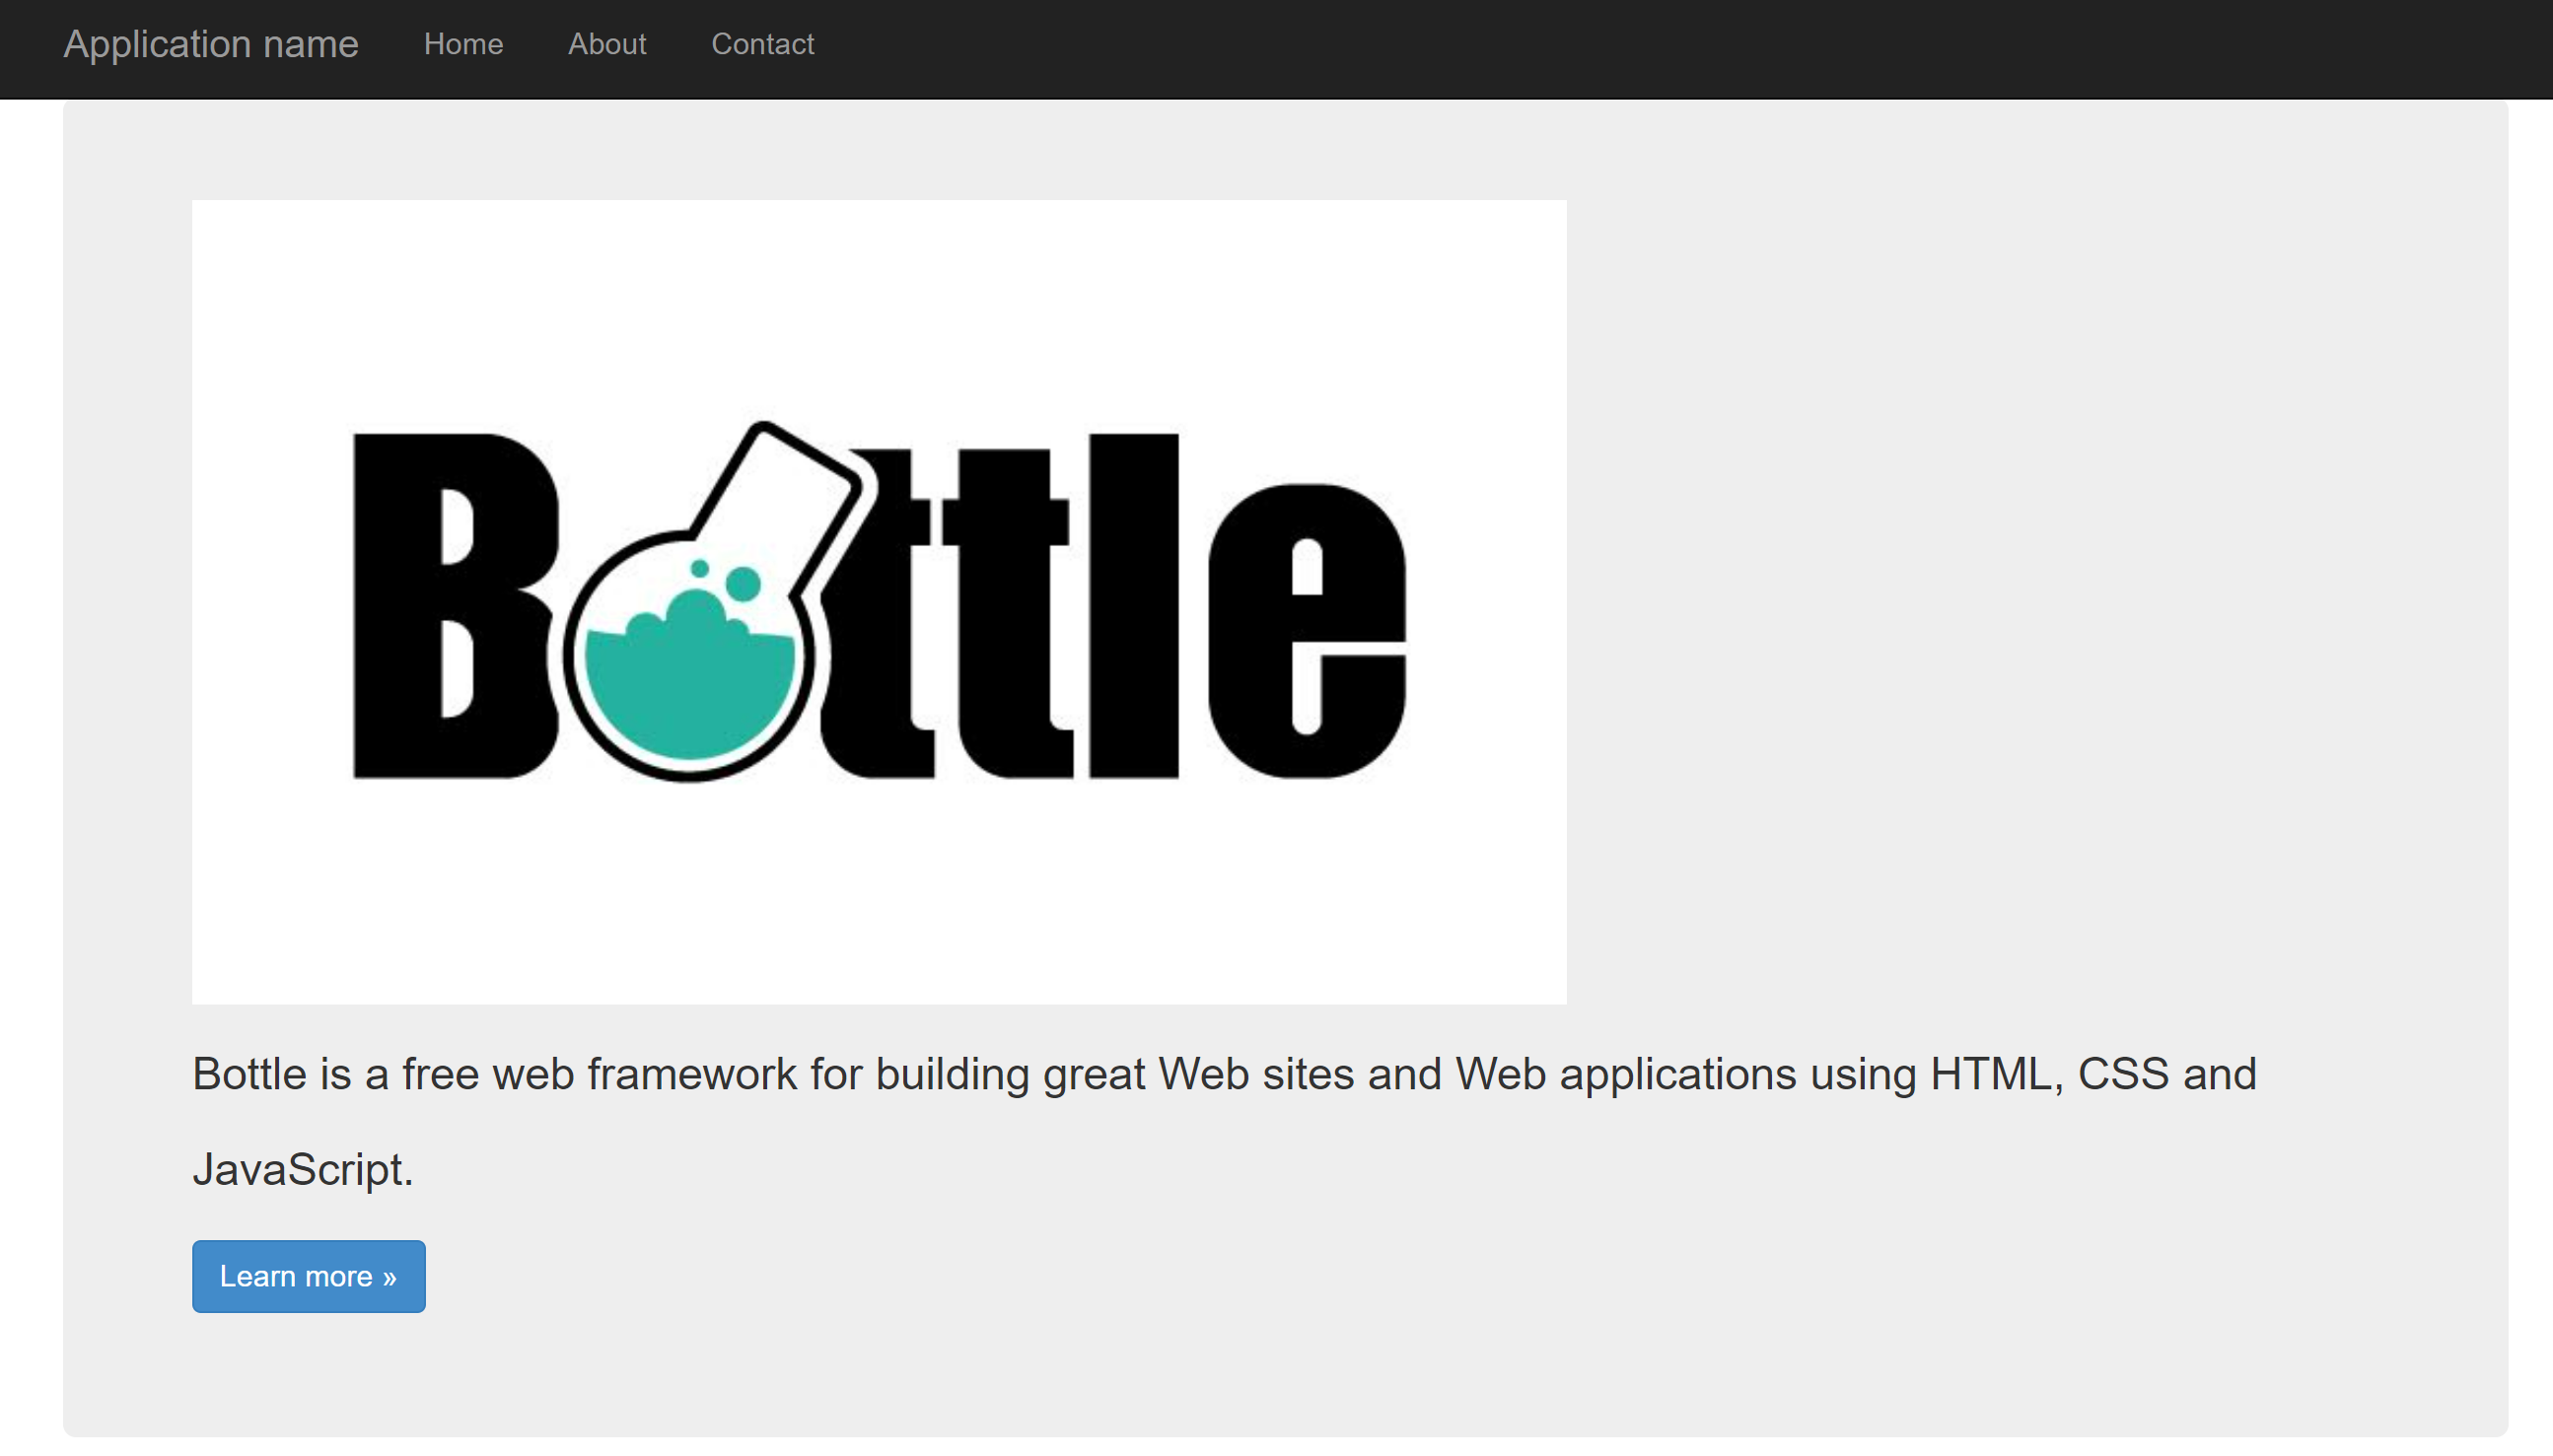
\includegraphics[width=.9\linewidth]{images/20230323-122110_screenshot.png}
\caption{Отображение сайта}
\end{figure}

\begin{figure}[H]
\centering
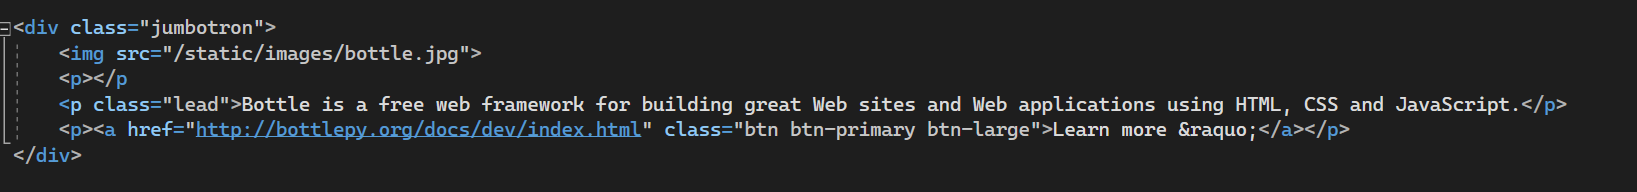
\includegraphics[width=.9\linewidth]{images/20230323-122156_screenshot.png}
\caption{Изменения кода}
\end{figure}


​6. Требуется создать веб-приложение (тематический сайт) на основе шаблона фреймворка Bottle. Придерживаться следующих этапов:  

\begin{itemize}
\item Выбрать тематику приложения, согласовать с преподавателем (темы не повторяются!).

ReportViwer - сайт для просмотра отчётов

\item Подобрать текстовые и графические (иллюстрации, иконки, карты) материалы для сайта.

Был разработан дизайн в Figma:

\begin{figure}[H]
\centering
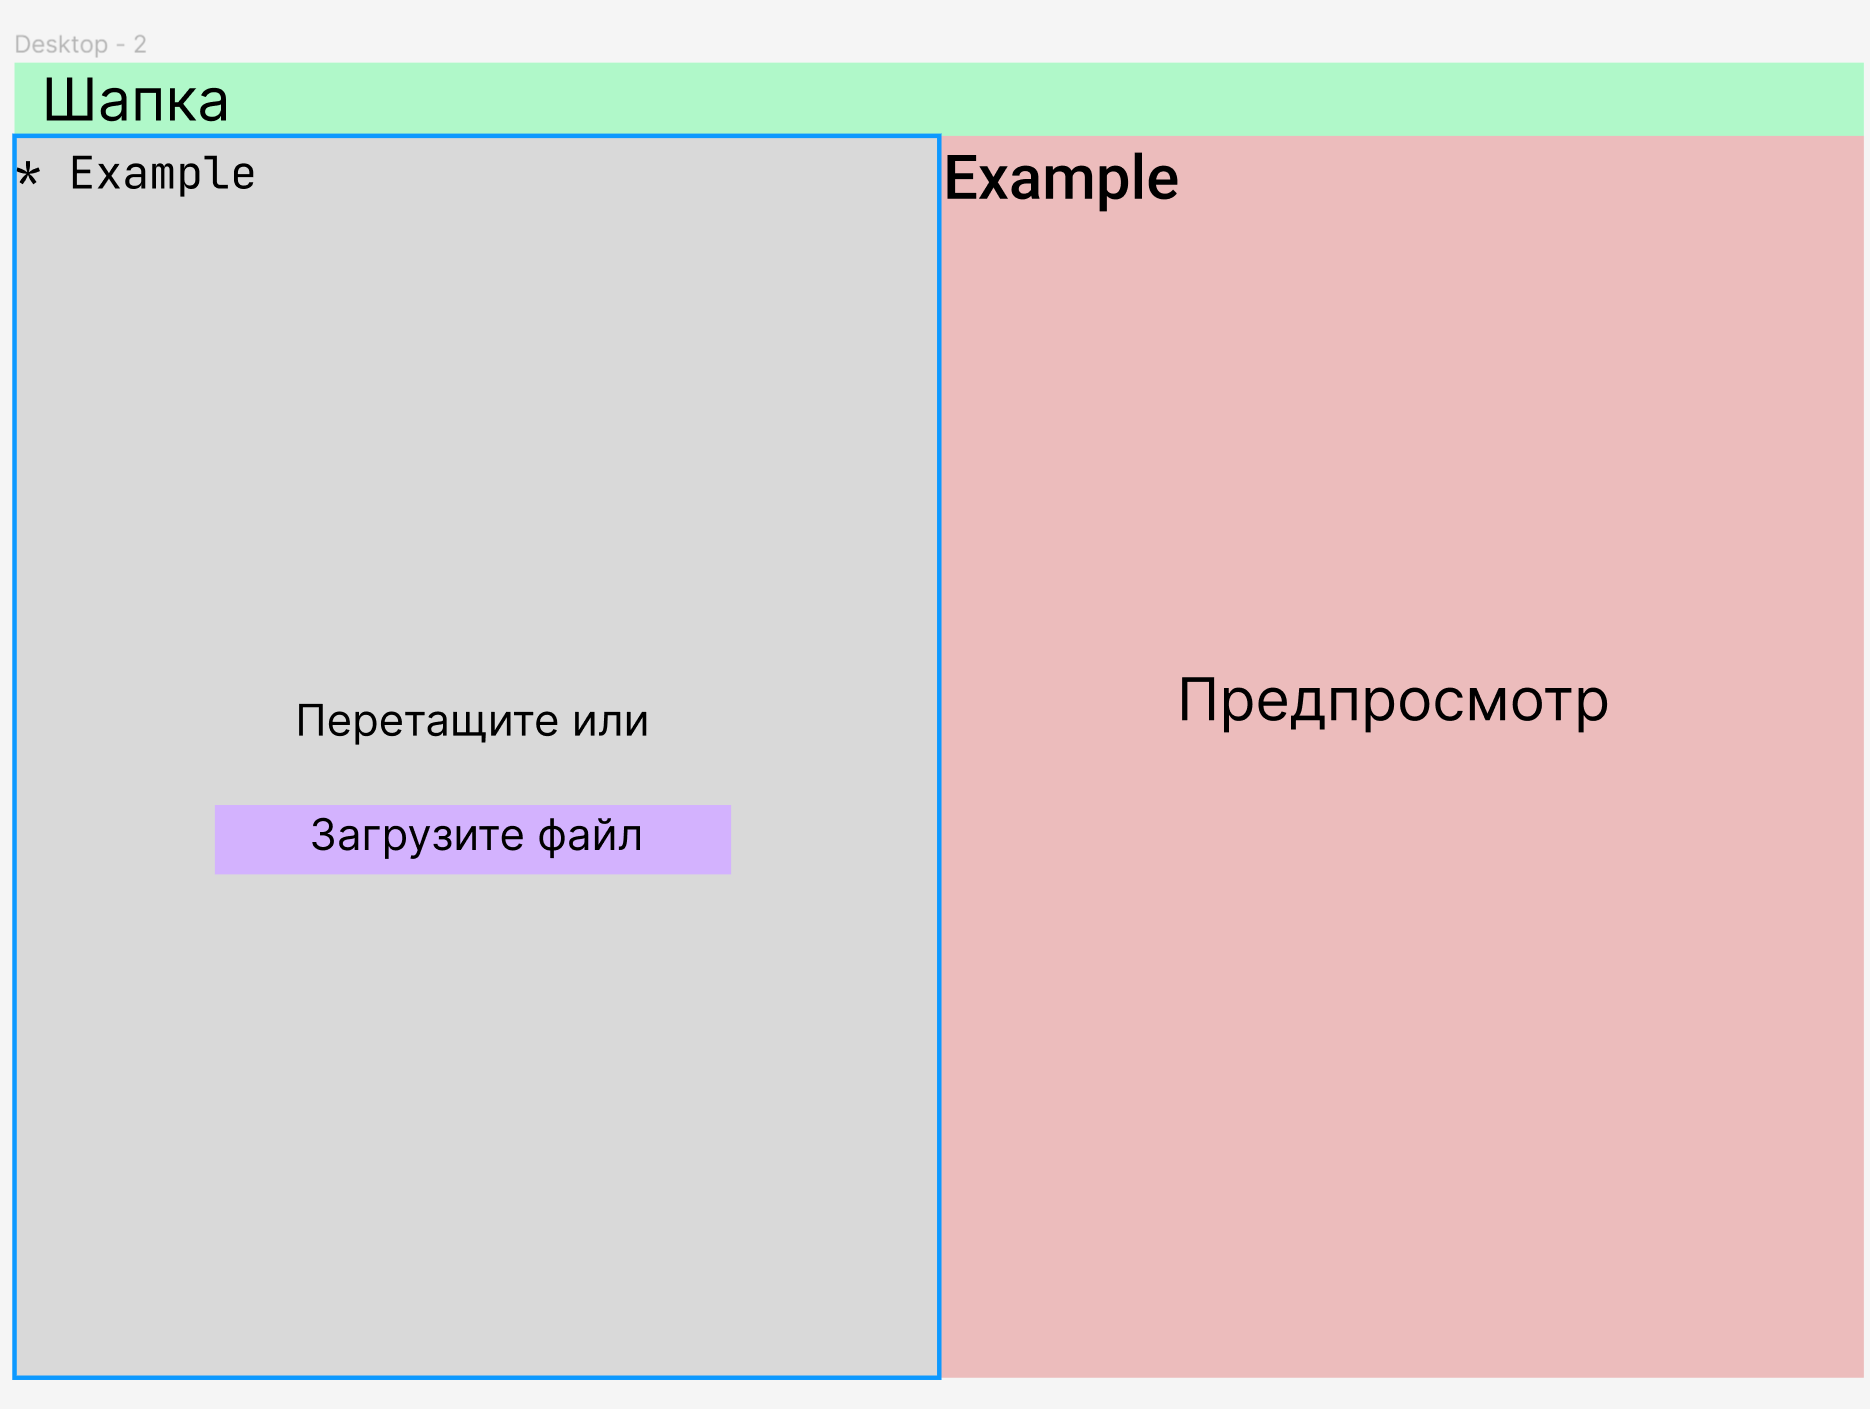
\includegraphics[width=.9\linewidth]{images/20230323-122737_screenshot.png}
\caption{Warframe}
\end{figure}
\end{itemize}


\begin{figure}[H]
\centering
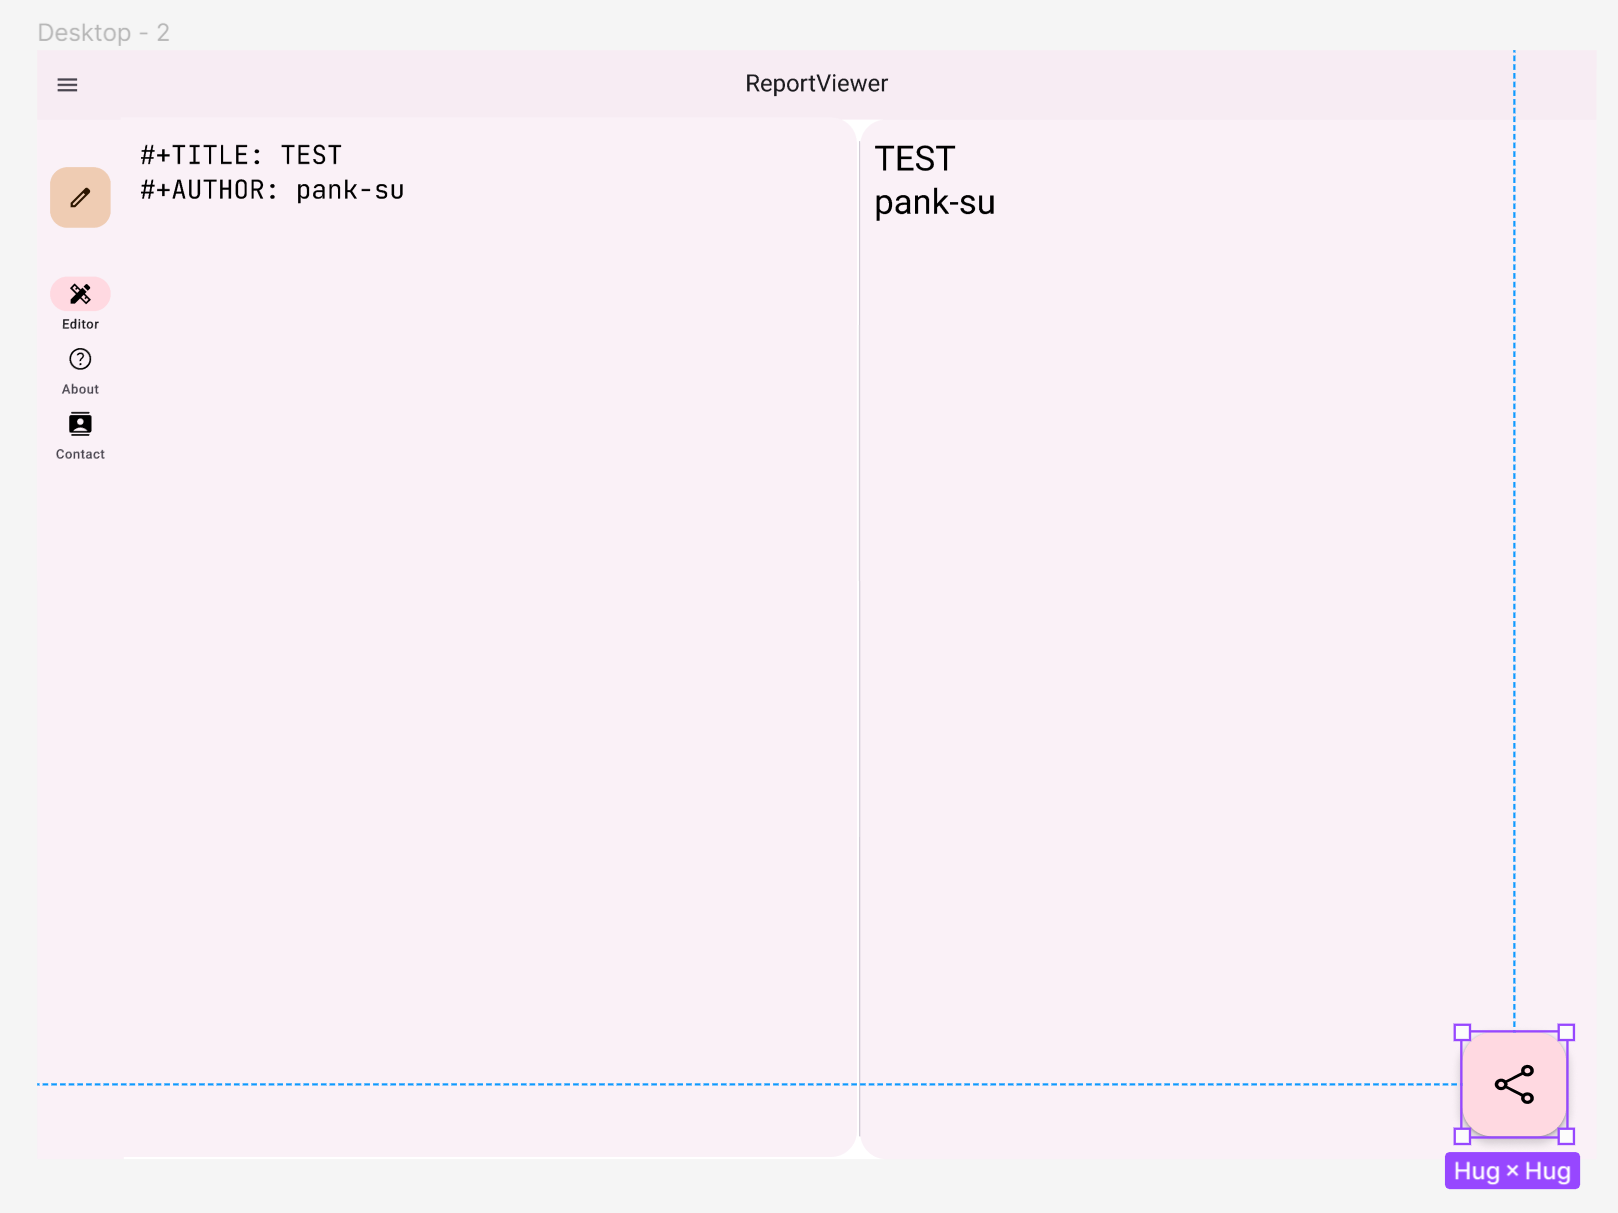
\includegraphics[width=.9\linewidth]{images/20230323-122438_screenshot.png}
\caption{Дизайн в Figma}
\end{figure}



\begin{itemize}
\item Построить UML-диаграмму компонентов приложения (css-файлы считать одним укрупнённым структурным компонентом, аналогично js-скрипты, их подключение осуществляется в файле layout.tpl).

\begin{figure}[H]
\centering
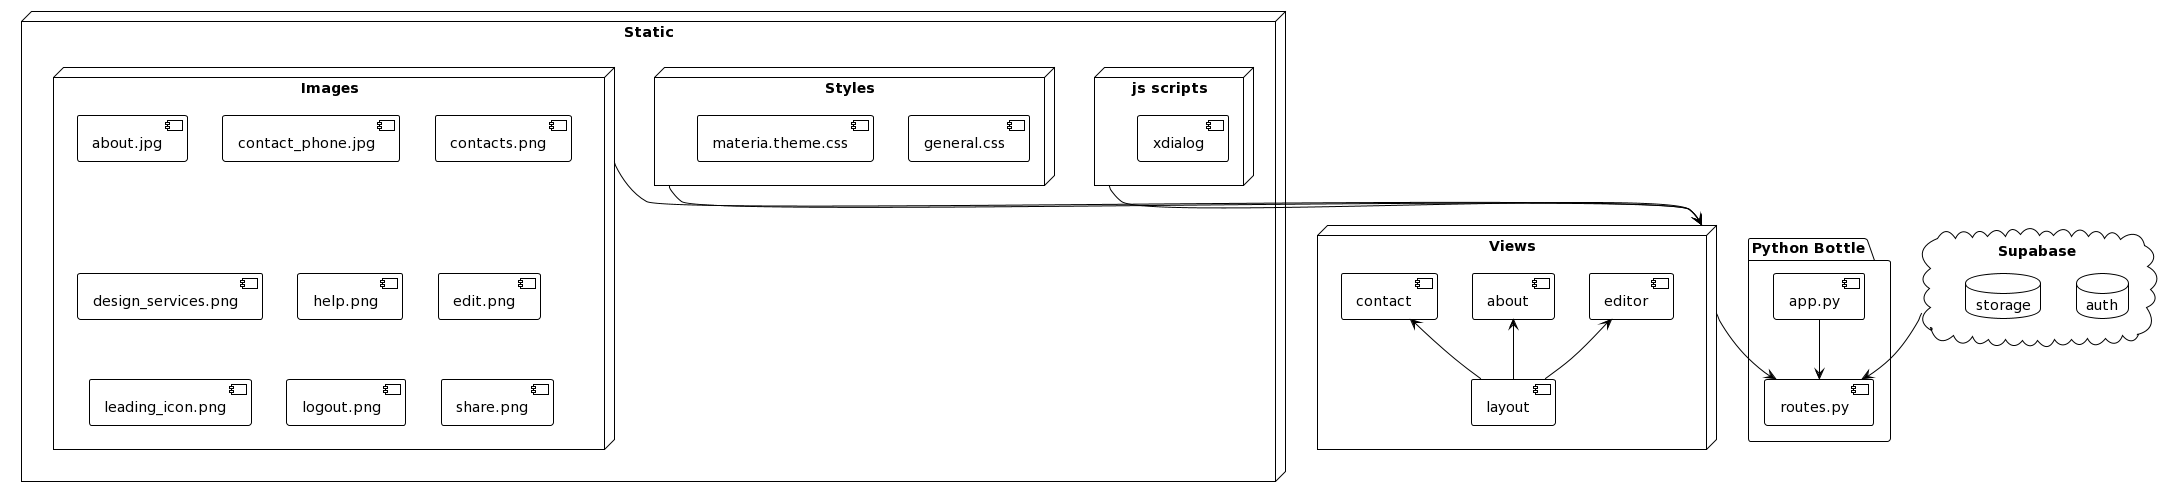
\includegraphics[width=.9\linewidth]{images/2023-04-05_10-35-52_screenshot.png}
\caption{UML-диаграммы}
\end{figure}
\end{itemize}


\begin{itemize}
\item Настроить Git. Хранение проекта осуществлять в репозитории на Github одного из участников, остальные клонируют проект в свой локальный репозиторий. Распределить задачи редактирования файлов шаблонов между членами команды. Изменить содержимое этих файлов согласно выбранной тематике (ссылки на кнопках поставить на нужные страницы похожих по тематике сайтов).

Репозитоий был создан мной на GitHub

\begin{center}

\includegraphics[width=.9\linewidth]{images/2023-04-05_09-33-51_screenshot.png}
\end{center}

\item Вести контроль версий. Синхронизировать все локальные изменения с удалённым репозиторием на Github.

В итоге были получены такие изменения от всех пользователей:
\begin{figure}[H]
\centering
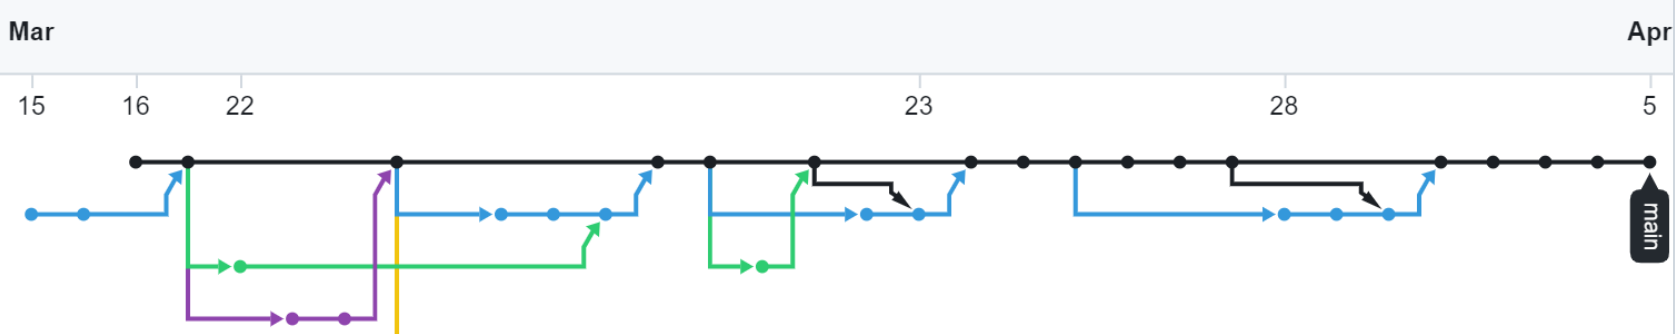
\includegraphics[width=.9\linewidth]{images/2023-04-05_09-35-15_screenshot.png}
\caption{Изменения от всех пользователей}
\end{figure}

Моя часть работы состояла, в создание основной части приложения, то есть редактора текстовых документов:
\begin{itemize}
\item Вид без авторизации:

\begin{figure}[H]
\centering
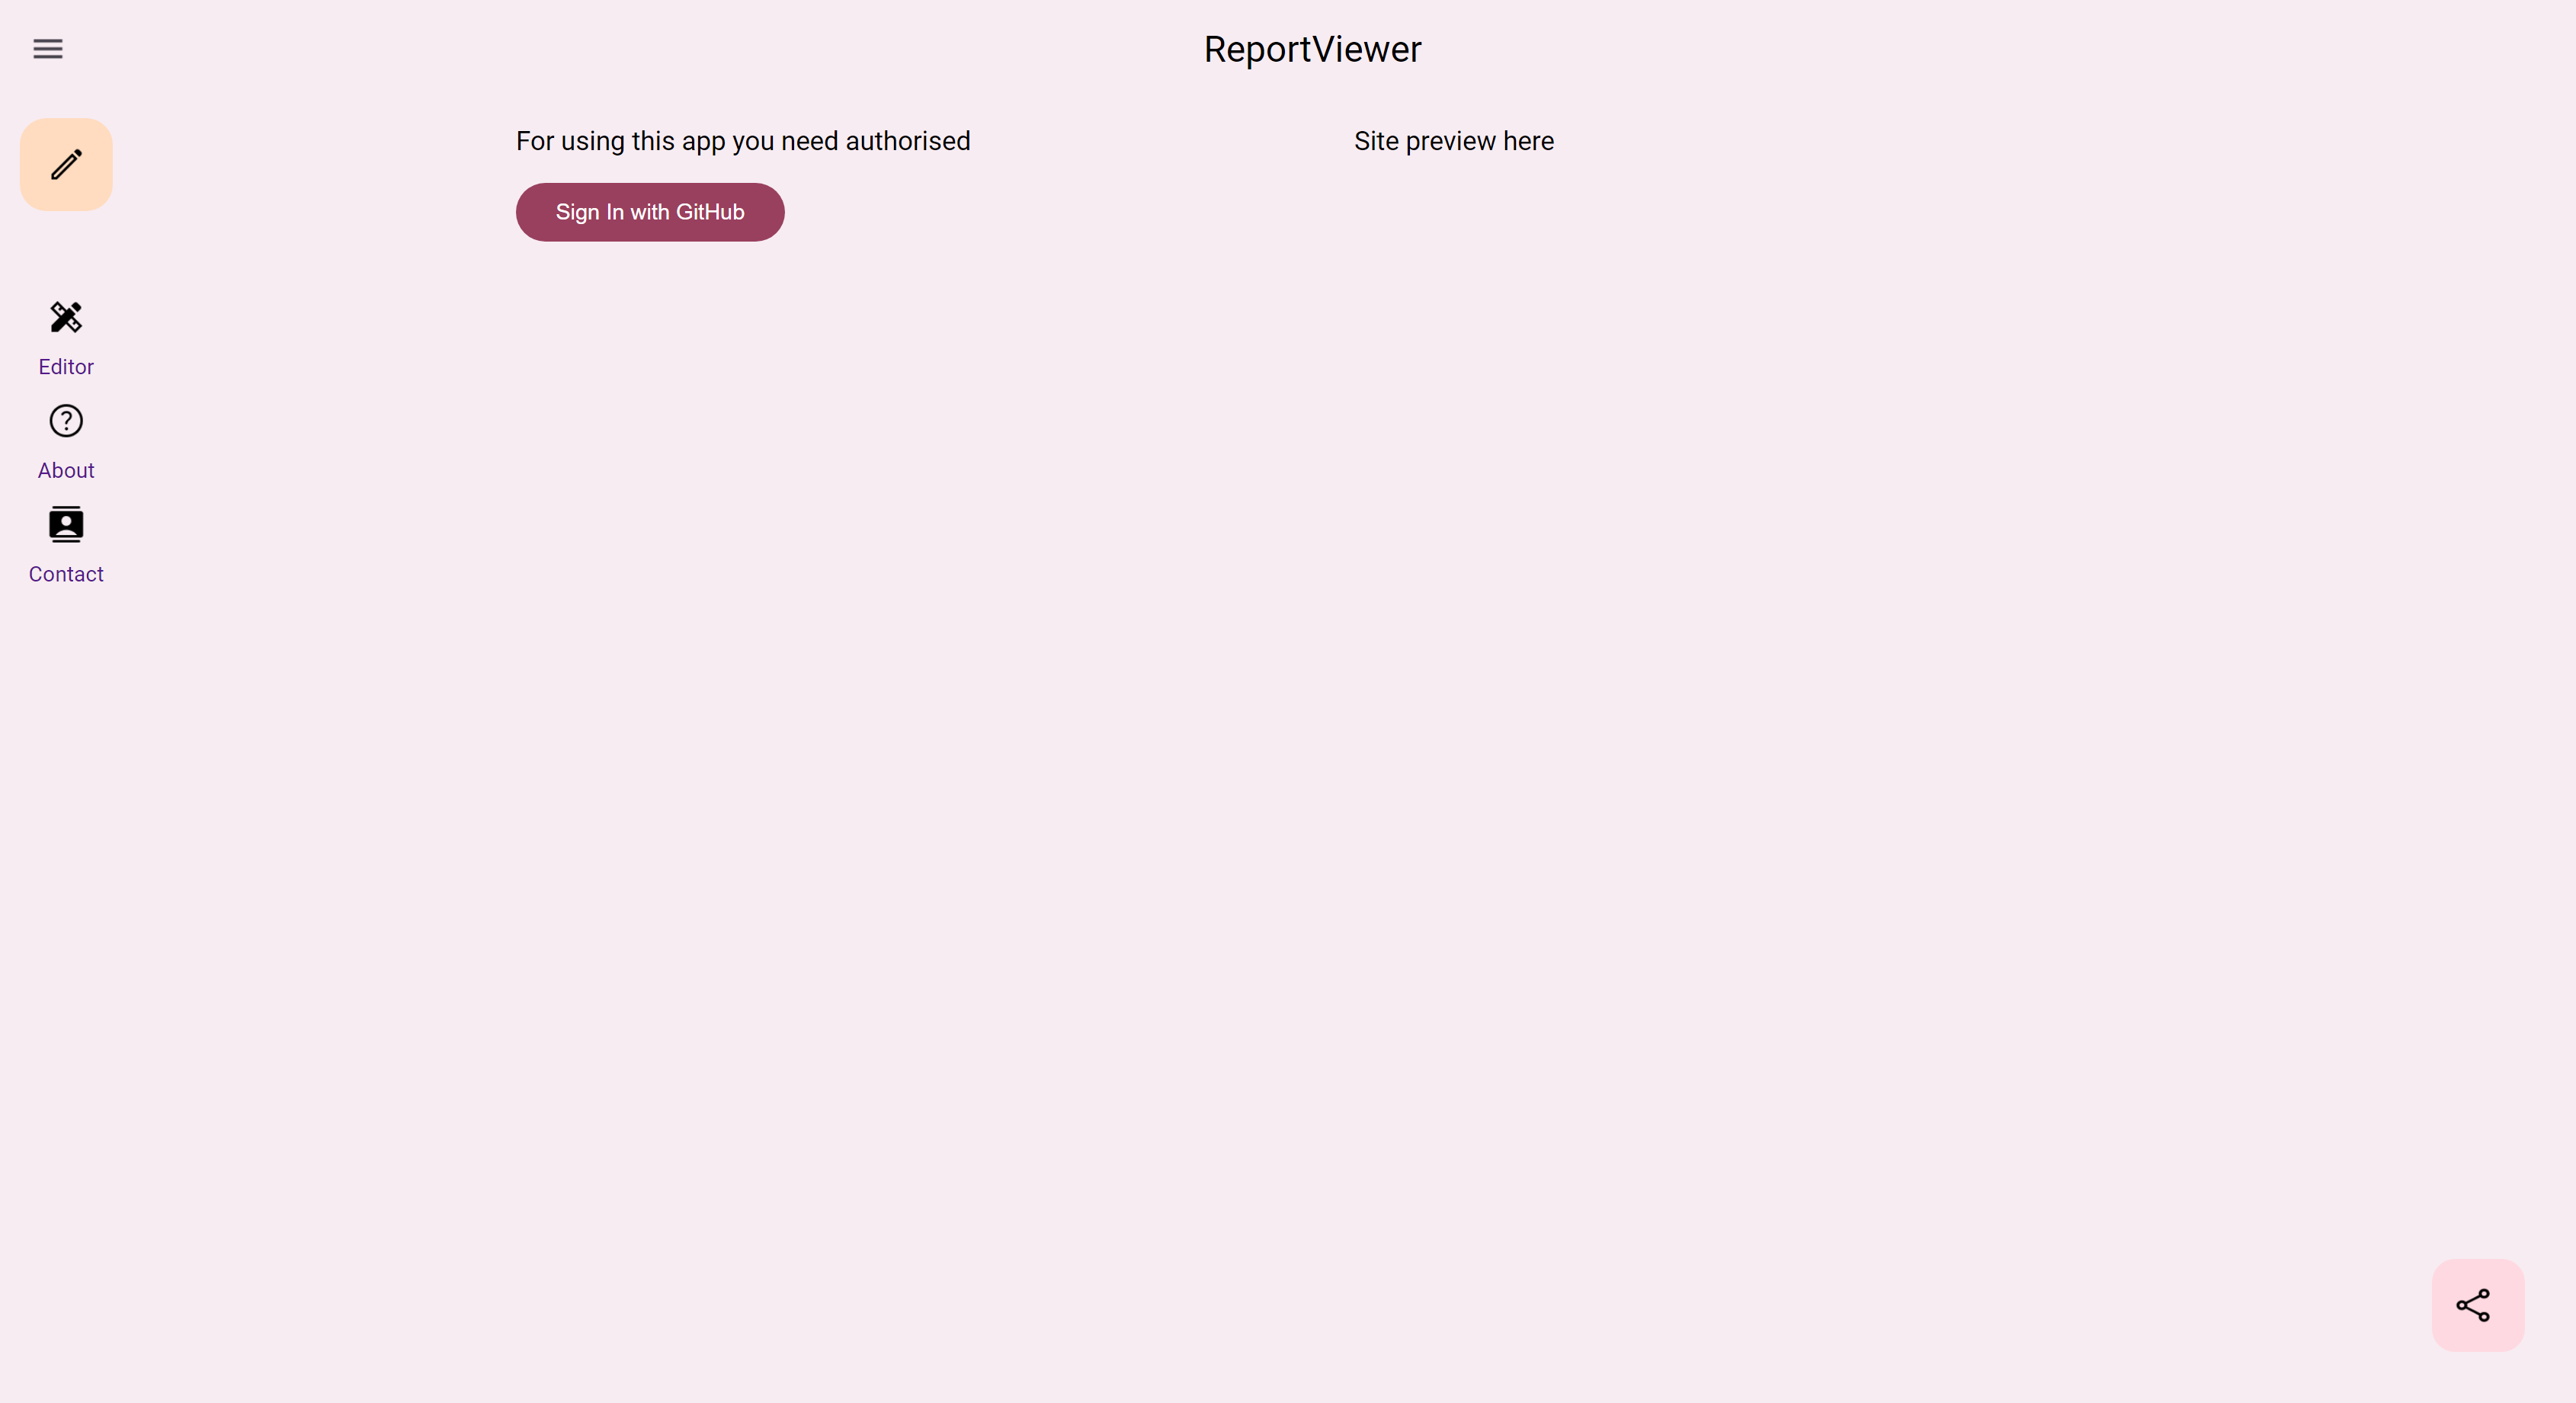
\includegraphics[width=.9\linewidth]{images/2023-04-05_09-41-07_screenshot.png}
\caption{Вид, без авторизации}
\end{figure}

\item Вид, после авторизации, с выбранным файлом
\begin{figure}[H]
\centering
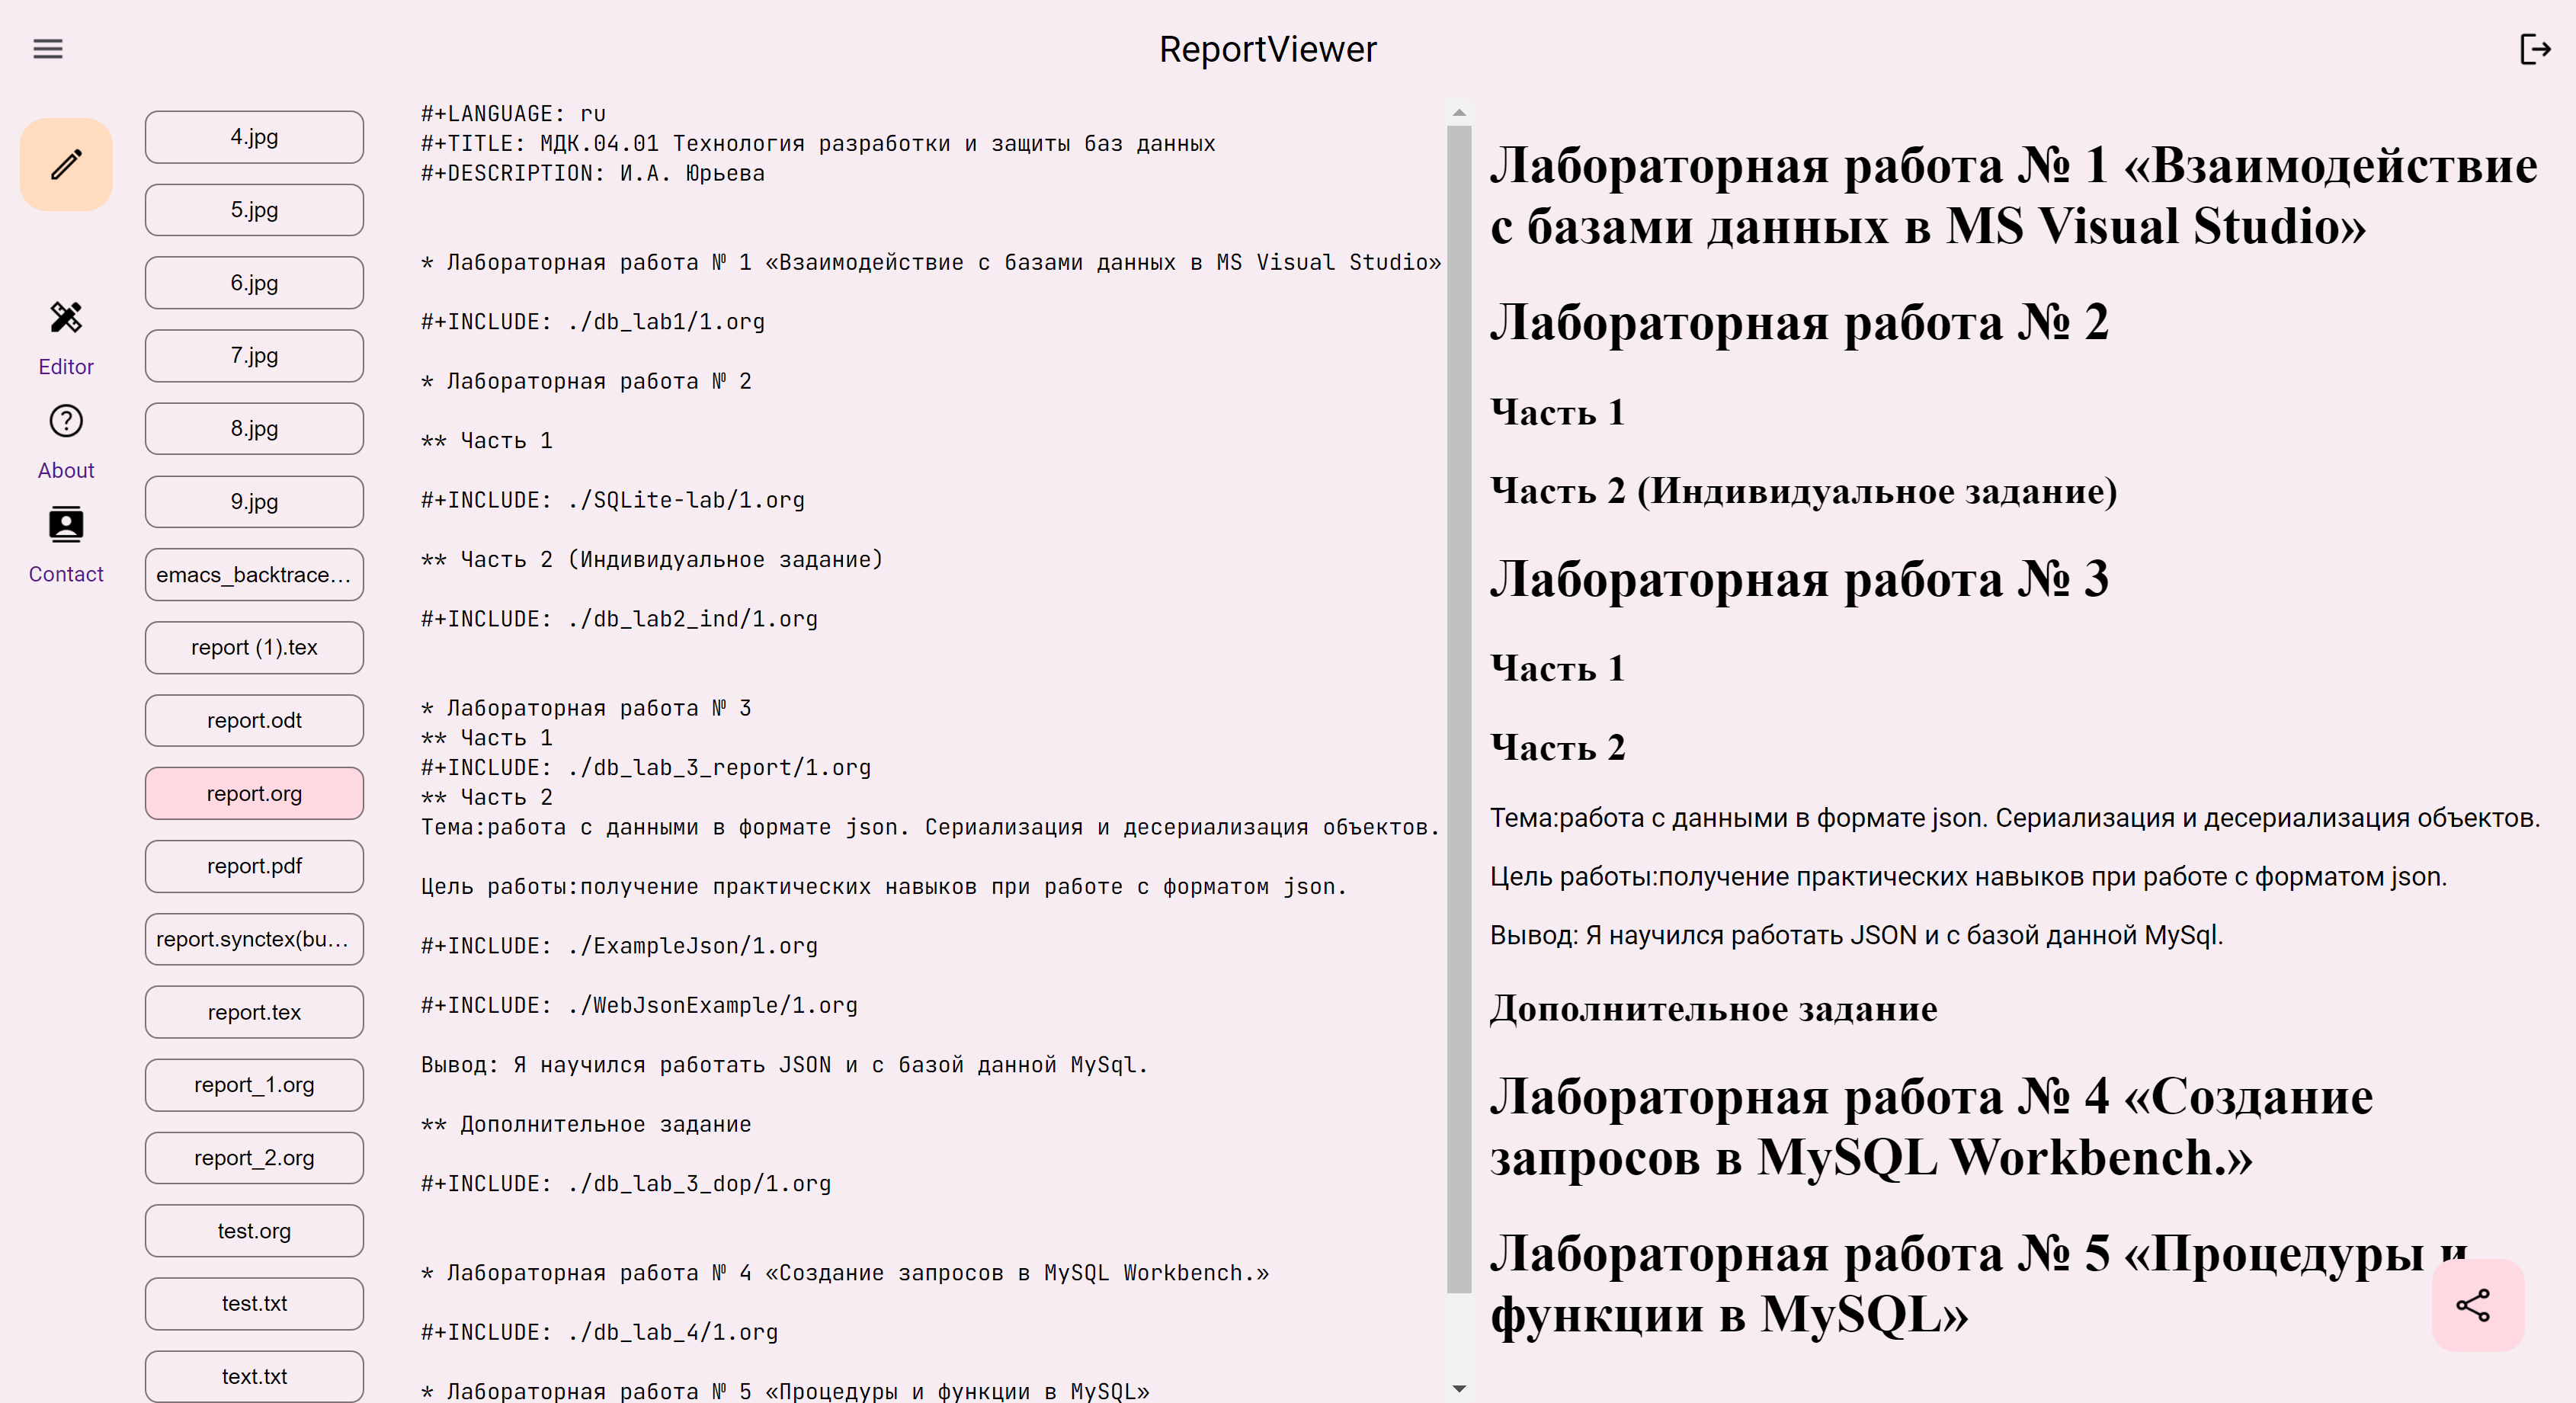
\includegraphics[width=.9\linewidth]{images/2023-04-05_09-42-23_screenshot.png}
\caption{Просмотр текстового файла}
\end{figure}

\item Просмотр картинки
\begin{figure}[H]
\centering
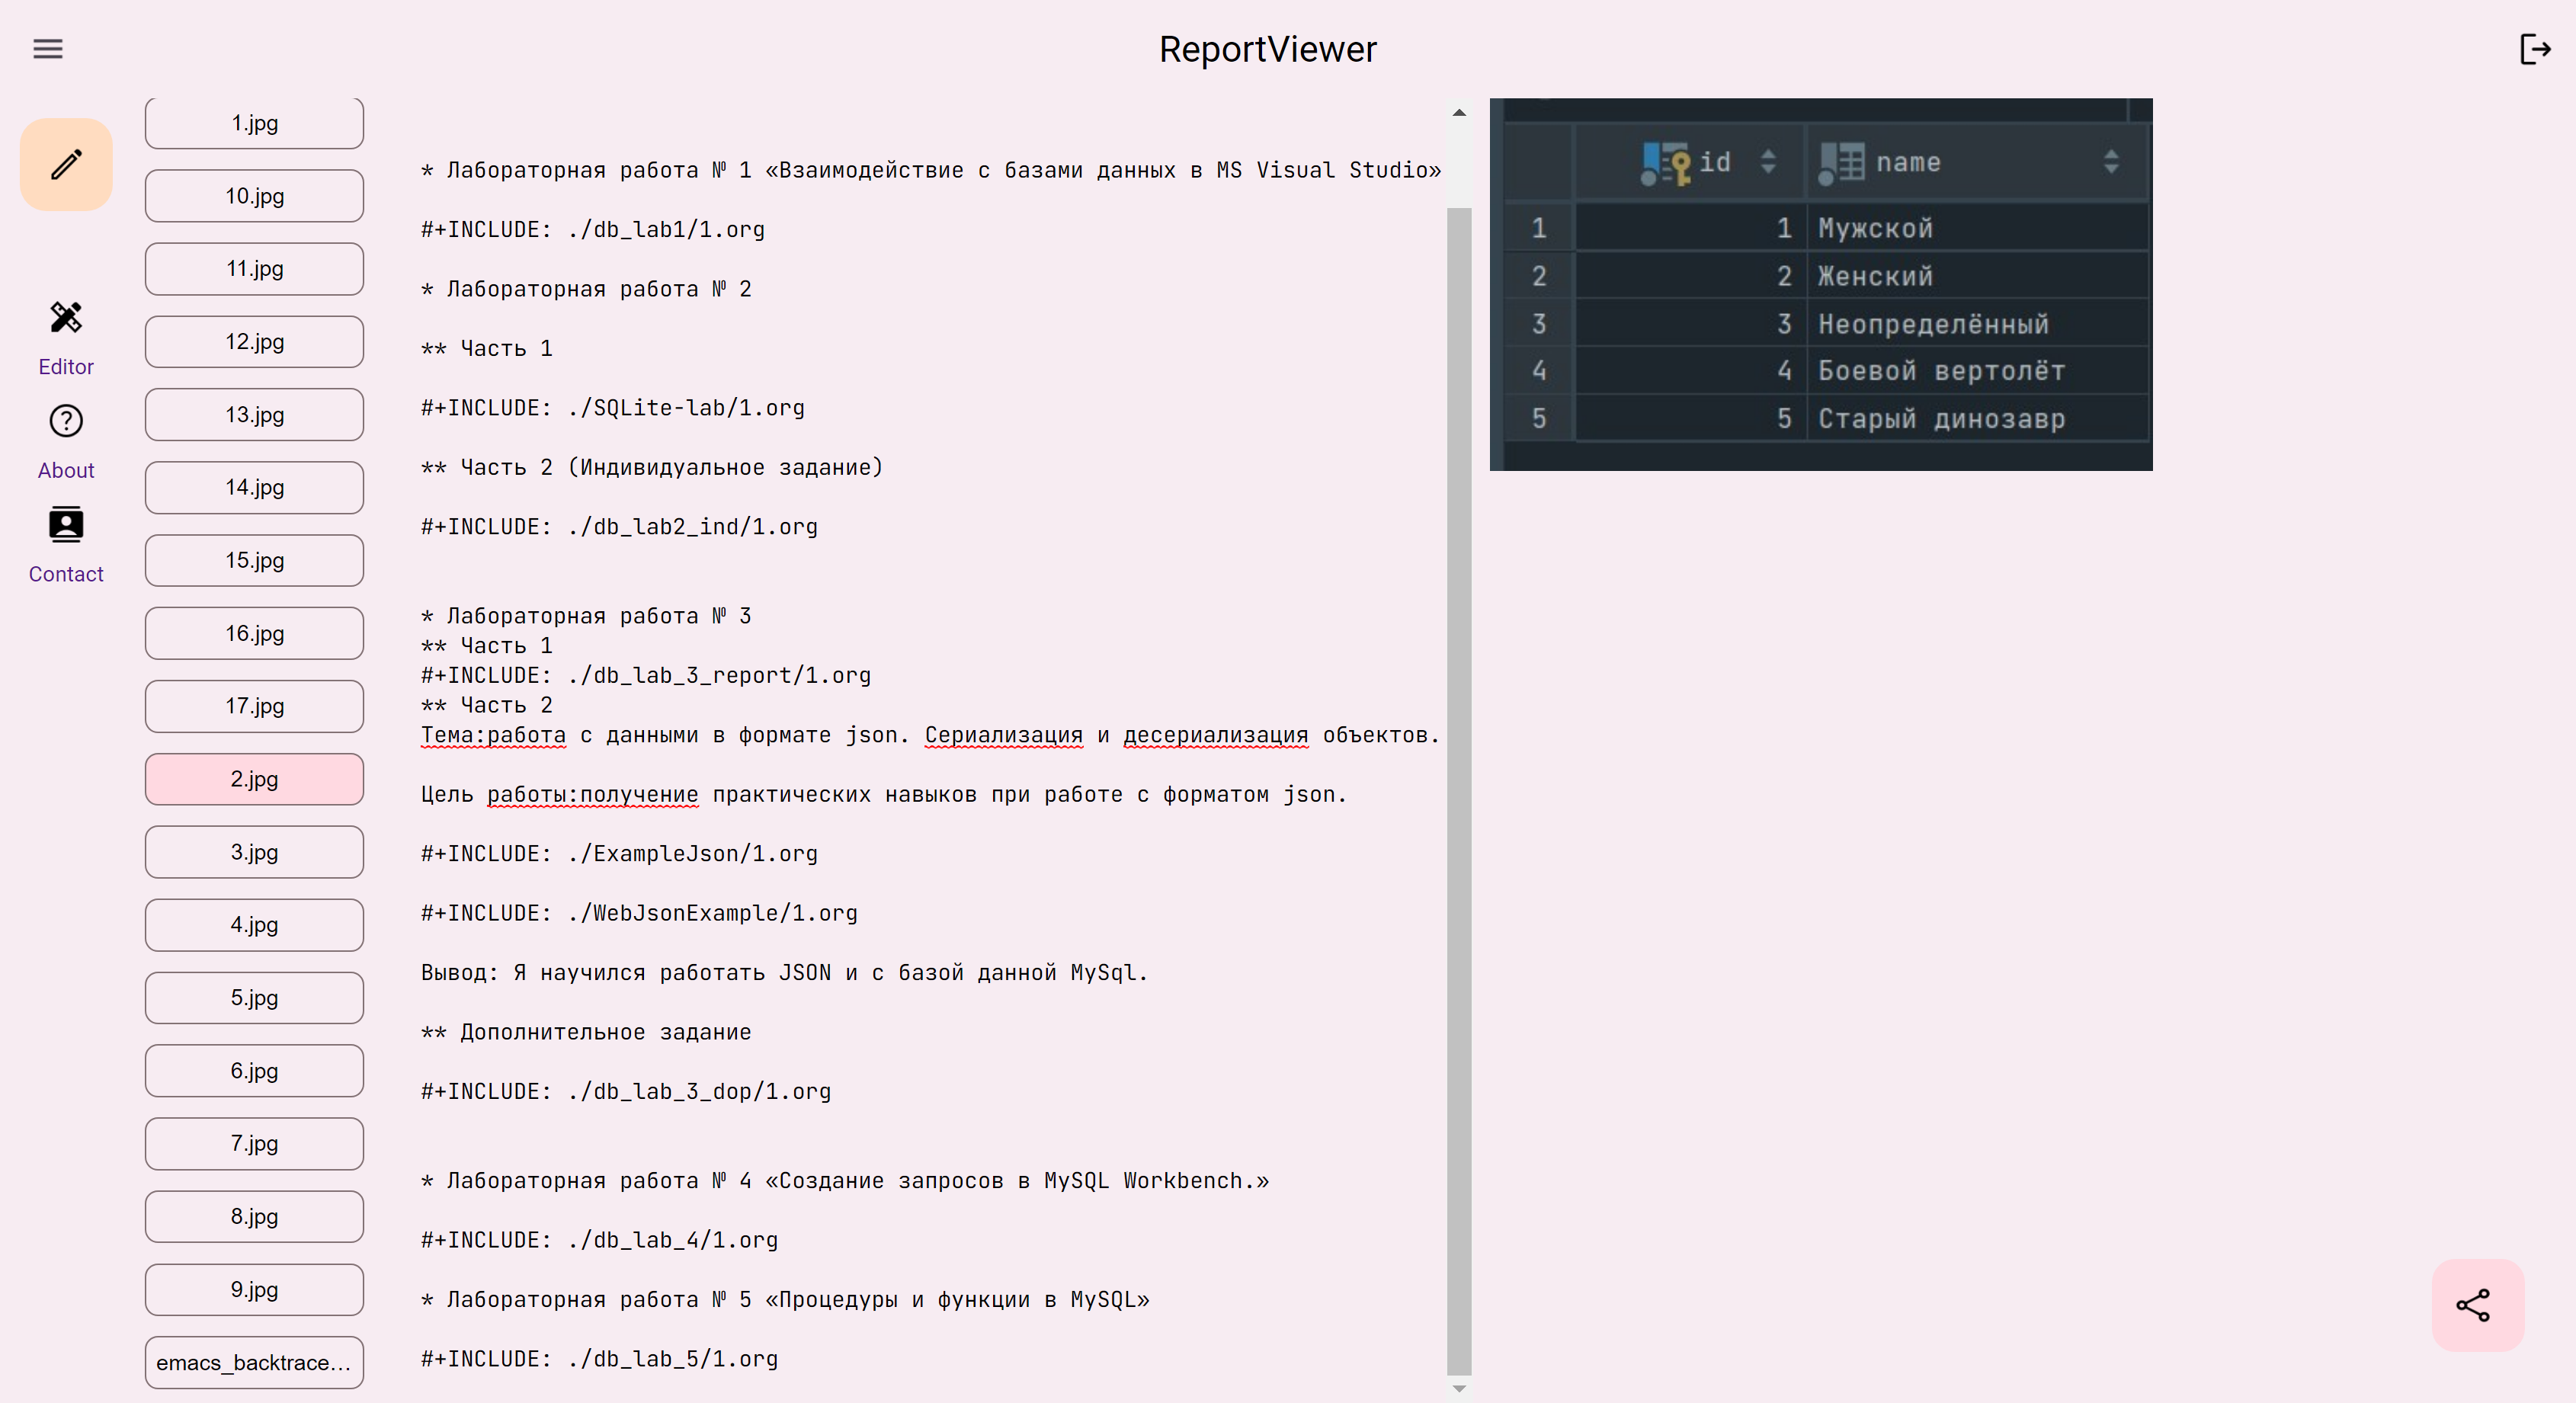
\includegraphics[width=.9\linewidth]{images/2023-04-05_09-43-05_screenshot.png}
\caption{Просмотр картинок}
\end{figure}
\end{itemize}

\item Заполнить файл README.md. Примерный вариант описания можно найти в шаблоне \url{https://gist.github.com/PurpleBooth/109311bb0361f32d87a2} или по ссылке \url{https://github.com/Sinclear/default\_readme}
\begin{figure}[H]
\centering
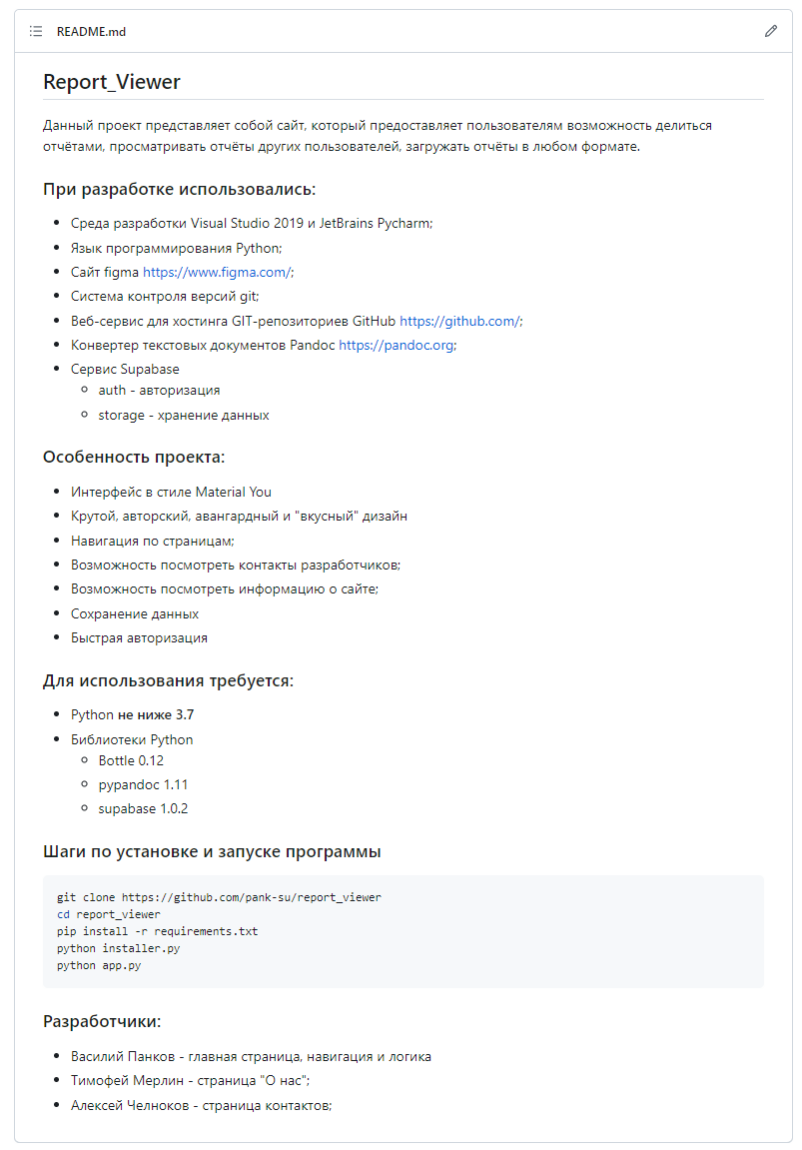
\includegraphics[width=.9\linewidth]{images/2023-04-05_10-36-38_screenshot.png}
\caption{README файл}
\end{figure}
\end{itemize}


Листинг программы:

app.py

\begin{Code}
\begin{Verbatim}
\color{EFD}\EFd{"""
This script runs the application using a development server.
"""}

\EFk{import} bottle
\EFk{import} os
\EFk{import} sys

\EFcd{\# }\EFc{routes contains the HTTP handlers for our server and must be imported. **NOT DELETE**}
\EFk{import} routes

\EFk{if} \EFs{'--debug'} \EFk{in} sys.argv[1:] \EFk{or} \EFs{'SERVER\_DEBUG'} \EFk{in} os.environ:
    \EFcd{\# }\EFc{Debug mode will enable more verbose output in the console window.}
    \EFcd{\# }\EFc{It must be set at the beginning of the script.}
    bottle.debug(\EFo{True})


\EFk{def} \EFf{wsgi\_app}():
    \EFd{"""Returns the application to make available through wfastcgi. This is used
    when the site is published to Microsoft Azure."""}
    \EFk{return} bottle.default\_app()


\EFk{if} \EFb{\_\_name\_\_} == \EFs{'\_\_main\_\_'}:
    \EFv{PROJECT\_ROOT} = os.path.abspath(os.path.dirname(\_\_file\_\_))
    \EFv{STATIC\_ROOT} = os.path.join(PROJECT\_ROOT, \EFs{'static'}).replace(\EFs{'}\EFo{\char92{}\char92{}}\EFs{'}, \EFs{'/'})
    \EFv{HOST} = os.environ.get(\EFs{'SERVER\_HOST'}, \EFs{'localhost'})
    \EFk{try}:
        \EFv{PORT} = \EFb{int}(os.environ.get(\EFs{'SERVER\_PORT'}, \EFs{'5555'}))
    \EFk{except} \EFt{ValueError}:
        \EFv{PORT} = 5555


    \EFt{@bottle.route}(\EFs{'/static/<filepath:path>'})
    \EFk{def} \EFf{server\_static}(filepath):
        \EFd{"""Handler for static files, used with the development server.
        When running under a production server such as IIS or Apache,
        the server should be configured to serve the static files."""}
        \EFk{return} bottle.static\_file(filepath, root=STATIC\_ROOT)


    \EFcd{\# }\EFc{Starts a local test server.}
    bottle.run(server=\EFs{'wsgiref'}, host=HOST, port=PORT)
\end{Verbatim}
\end{Code}

routes.py

\begin{Code}
\begin{Verbatim}
\color{EFD}\EFd{"""
Routes and views for the bottle application.
"""}
\EFk{import} os
\EFk{import} shutil
\EFk{from} datetime \EFk{import} datetime

\EFk{import} pypandoc
\EFk{import} storage3.utils
\EFk{from} bottle \EFk{import} route, view, request, response, FileUpload, BaseRequest, redirect, HTTPResponse
\EFk{from} supabase \EFk{import} create\_client, Client

BaseRequest.\EFv{MEMFILE\_MAX} = 1024 * 1024  \EFcd{\# }\EFc{ограничение по памяти}

\EFv{url}: \EFb{str} = os.environ.get(\EFs{"SUPABASE\_URL"})
\EFv{key}: \EFb{str} = os.environ.get(\EFs{"SUPABASE\_KEY"})

\EFv{supabase}: Client = create\_client(url, key)

\EFcd{\# }\EFc{переменная, содержащая секретный ключ, используемый для защиты куков}
\EFv{SECRET} = os.environ.get(\EFs{"SECRET\_TOKEN"})
\EFcd{\# }\EFc{это переменная, содержащая путь к директории, в которой будут храниться файлы превью}
\EFv{savable\_path} = \EFs{"./save/"}
\EFv{temporary\_path} = \EFs{"./temp/"}


\EFk{def} \EFf{check\_path}(path: \EFb{str}) -> \EFo{None}:
    \EFd{"""Функция, которая проверяет есть ли путь, если нет, то создаёт его"""}
    \EFk{if} \EFk{not} os.path.exists(path):
        os.makedirs(path)


check\_path(savable\_path)


\EFt{@route}(\EFs{'/'})
\EFt{@route}(\EFs{'/editor'})
\EFt{@view}(\EFs{'editor'})
\EFk{def} \EFf{editor}():
    \EFv{query} = request.query
    \EFv{user\_id} = \EFo{None}
    \EFk{if} request.query\_string != \EFs{""}:
        \EFk{try}:
            supabase.auth.refresh\_session(query[\EFs{"refresh\_token"}])
            \EFv{user\_id} = supabase.auth.get\_user().user.\EFb{id}
        \EFk{except} \EFt{Exception} \EFk{as} e:
            \EFv{user\_id} = \EFo{None}
        \EFk{if} user\_id \EFk{is} \EFo{None}:
            supabase.auth.set\_session(query[\EFs{"access\_token"}])
    \EFk{elif} user\_id \EFk{is} \EFo{None}:
        \EFk{try}:
            \EFv{user\_id} = request.get\_cookie(\EFs{"user\_id"}, secret=SECRET)
        \EFk{except} \EFt{Exception} \EFk{as} e:
            \EFv{user\_id} = \EFo{None}
    \EFk{if} user\_id \EFk{is} \EFk{not} \EFo{None}:
        response.set\_cookie(\EFs{"user\_id"}, user\_id, secret=SECRET)
        \EFk{try}:
            supabase.storage.create\_bucket(user\_id)
        \EFk{except} storage3.utils.StorageException:
            \EFk{pass}
        \EFv{storage} = supabase.storage.get\_bucket(user\_id)
        \EFk{if} \EFb{len}(storage.\EFb{list}()) == 0:
            storage.upload(\EFs{"test.org"}, \EFs{"./tested\_file/test.org"})
        \EFk{return} \EFb{dict}(
            year=datetime.now().year,
            userExist=\EFo{True},
            files=storage.\EFb{list}(),
            user\_id=user\_id
        )
    \EFk{else}:
        \EFk{return} \EFb{dict}(
            year=datetime.now().year,
            userExist=\EFo{False},
            files=[],
            user\_id=\EFs{""}

        )


\EFt{@route}(\EFs{'/contact'})
\EFt{@view}(\EFs{'contact'})
\EFk{def} \EFf{contact}():
    \EFd{"""Renders the contact page."""}
    \EFk{return} \EFb{dict}(
        title=\EFs{'Contact'},
        year=datetime.now().year
    )


\EFt{@route}(\EFs{'/about'})
\EFt{@view}(\EFs{'about'})
\EFk{def} \EFf{about}():
    \EFd{"""Renders the about page."""}
    \EFk{return} \EFb{dict}(
        title=\EFs{'About us'},
        message=\EFs{'Here you can see the possibilities of our site'},
        year=datetime.now().year,
        functions=\EFs{'At this site you could:'},
        func1=\EFs{'share reports'},
        func2=\EFs{'watch reports'},
        func3=\EFs{'download reports'},
        func4=\EFs{'change report format'}
    )


\EFt{@route}(\EFs{'/upload'}, method=\EFs{'POST'})
\EFk{def} \EFf{do\_upload}():
    \EFd{"""Обработчик маршрута, которая обрабатывает POST-запрос на загрузку файла. Она сохраняет загружxенный файл во
    временную директорию, конвертирует его в формат org с помощью pypandoc, генерирует случайный хэш-код и сохраняет
    конвертированный файл с использованием этого хэш-кода в постоянную директорию"""}
    \EFv{upload}: FileUpload = request.files.get(\EFs{'file'})
    check\_path(temporary\_path)
    upload.save(temporary\_path + upload.filename)
    \EFv{org\_text} = pypandoc.convert\_file(temporary\_path + upload.filename, \EFs{'org'})
    \EFv{user\_id} = request.get\_cookie(\EFs{"user\_id"}, SECRET)
    \EFv{save\_path} = savable\_path + user\_id + \EFs{"/"}
    \EFk{if} \EFk{not} os.path.exists(save\_path):
        os.makedirs(save\_path)
    \EFv{filename} = \EFs{"."}.join(upload.filename.split(\EFs{'.'})[:-1]) + \EFs{".org"}
    \EFv{new\_filename} = filename
    \EFk{with} \EFb{open}(savable\_path + user\_id + \EFs{"/"} + filename, \EFs{"w"}, encoding=\EFs{"utf-8"}) \EFk{as} f:
        f.write(org\_text)
    shutil.rmtree(temporary\_path)
    \EFv{is\_sent} = \EFo{False}
    \EFv{file\_id} = 0
    \EFk{while} \EFk{not} is\_sent:
        \EFk{try}:
            supabase.storage.get\_bucket(user\_id).upload(new\_filename, savable\_path + user\_id + \EFs{"/"} + filename)
            \EFv{is\_sent} = \EFo{True}
        \EFk{except} storage3.utils.StorageException:
            \EFv{file\_id} += 1
            \EFv{new\_filename} = \EFs{"."}.join(upload.filename.split(\EFs{'.'})[:-1]) + f\EFs{"\_}\{file\_id\}\EFs{.org"}
    \EFk{return} \EFs{"ok"}


\EFk{def} \EFf{generate\_preview}(user\_id, filename):
    \EFd{"""Функция, которая генерирует превью"""}
    \EFv{save\_path} = savable\_path + user\_id + \EFs{"/"}
    check\_path(save\_path)
    \EFk{with} \EFb{open}(save\_path + filename, \EFs{"wb"}) \EFk{as} f:
        \EFv{res} = supabase.storage.from\_(user\_id).download(filename)
        f.write(res)
    \EFv{html\_text} = \EFs{"С файлом что-то не так"}
    \EFk{try}:
        \EFv{html\_text} = pypandoc.convert\_file(save\_path + filename, \EFs{'html'})
    \EFk{except} \EFt{RuntimeError}:
        \EFs{"""Если файл не текст"""}
        \EFv{url} = supabase.storage.from\_(user\_id).get\_public\_url(filename)
        \EFv{html\_text} = f\EFs{"<img src='}\{url\}\EFs{' />"}
    \EFk{return} html\_text


\EFt{@route}(\EFs{"/preview"})
\EFt{@view}(\EFs{"preview"})
\EFk{def} \EFf{preview}():
    \EFk{return} \EFb{dict}(
        previewContent=\EFs{"<p>Site preview here</p>"}
    )


\EFt{@route}(\EFs{'/preview/<filename>'})
\EFt{@view}(\EFs{"preview"})
\EFk{def} \EFf{preview}(filename):
    \EFv{user\_id} = request.get\_cookie(\EFs{"user\_id"}, secret=SECRET)
    \EFk{return} \EFb{dict}(previewContent=generate\_preview(user\_id, filename))


\EFt{@route}(\EFs{'/s/<user\_id>/<filename>'})
\EFt{@view}(\EFs{"preview"})
\EFk{def} \EFf{preview}(user\_id, filename):
    \EFk{return} \EFb{dict}(previewContent=generate\_preview(user\_id, filename))


\EFt{@route}(\EFs{"/preview\_reload"}, method=\EFs{'POST'})
\EFk{def} \EFf{preview\_reload}():
    \EFd{"""Обработчик маршрута, который вызывается при изменении содержимого файла пользователем в редакторе"""}
    \EFv{filename} = request.json[\EFs{"filename"}]
    \EFv{data} = request.json[\EFs{"data"}]
    \EFb{print}(data)
    \EFv{user\_id} = request.get\_cookie(\EFs{"user\_id"}, secret=SECRET)
    supabase.storage.from\_(user\_id).remove(filename)
    check\_path(temporary\_path)
    \EFk{with} \EFb{open}(temporary\_path + filename, \EFs{"w"}, encoding=\EFs{"utf-8"}) \EFk{as} f:
        f.write(data)
    supabase.storage.from\_(user\_id).upload(filename, temporary\_path + filename)

    \EFcd{\# }\EFc{shutil.rmtree(temporary\_path)}
    \EFk{return} \EFs{"ok"}


\EFt{@route}(\EFs{"/content/<filename>"})
\EFk{def} \EFf{get\_content}(filename: \EFb{str}):
    \EFd{"""Сохраняет файл в директории save\_path и возвращает значение"""}
    \EFk{if} filename.endswith((\EFs{".png"}, \EFs{".jpg"})):
        \EFk{return} HTTPResponse(status=400, body=\EFs{"This is not text"})
    \EFv{user\_id} = request.get\_cookie(\EFs{"user\_id"}, SECRET)
    \EFv{save\_path} = savable\_path + user\_id + \EFs{"/"}
    check\_path(save\_path)
    \EFk{if} user\_id \EFk{is} \EFo{None}:
        \EFk{return} \EFo{None}

    \EFk{with} \EFb{open}(save\_path + filename, \EFs{"wb"}) \EFk{as} f:
        \EFv{res} = supabase.storage.from\_(user\_id).download(filename)
        f.write(res)
    \EFk{try}:
        \EFk{with} \EFb{open}(save\_path + filename, \EFs{"r"}, encoding=\EFs{"utf-8"}) \EFk{as} f:
            \EFk{return} f.read()
    \EFk{except} \EFt{UnicodeDecodeError}:
        \EFk{return} HTTPResponse(status=400, body=\EFs{"This is not text"})


\EFt{@route}(\EFs{"/logout"})
\EFk{def} \EFf{logout}():
    supabase.auth.sign\_out()
    response.set\_cookie(\EFs{"user\_id"}, \EFs{""})
    redirect(\EFs{"/"})
\end{Verbatim}
\end{Code}

general.css

\begin{Code}
\begin{Verbatim}
\color{EFD}@import url('https://fonts.googleapis.com/css2?family=Roboto\&display=swap');
@import url('https://fonts.googleapis.com/css2?family=JetBrains+Mono\&display=swap');
@import url('../material-theme/theme.css');

.myAppBar \{
    display: flex;
    flex-direction: row;
    align-items: center;

    gap: 6px;
    height: 7\%;
\}

:root p \{
    font-family: "Roboto";
\}

.title \{
    text-align: center;
    margin: auto;
    padding-right: 24px;
\}

body \{
    margin: 0;
\}

.icon-button \{
    background: transparent;
    border: none;
    height: 48px;
    justify-content: center;
    align-items: center;
    width: 48px;
    display: flex;
    flex-direction: column;
\}

.icon-button img \{
    height: 46px;
    width: 46px;
    margin: auto;
\}

/*Тут будет крутой hovered эффект*/
.icon-button img:hover \{
    background: \#49454F14;
    background-size: 48px;
    border-radius: 50\%;
\}

.navigation-rail \{
    display: flex;
    flex-direction: column;
    align-items: flex-start;
    padding: 0 0 -56px;
    width: 80px;
    height: 100\%;
\}

.fab \{
    display: flex;
    flex-direction: row;
    align-items: flex-start;
    width: 56px;
    height: 56px;
    margin: 12px;
    border: none;
    border-radius: 16px;
\}

.fab img \{
    margin: auto;
    width: 24px;
    height: 24px;
\}

.fab:hover \{
    background: \#EFCCB3;

\}

.navs \{
    display: flex;
    flex-direction: column;
    justify-content: center;
    align-items: center;
    width: 56px;
    margin: 40px 12px 12px;
\}

.icon \{
    width: 24px;
    height: 24px;
\}

.naaav \{
    display: flex;
    flex-direction: column;
    align-items: center;
    margin: auto;
\}

.nav.active img \{

\}

.nav p \{
    /*font-weight: bold;*/
    margin-top: 10px;
    font-size: 13px;
\}

.nav:link \{
    text-decoration: none;
\}

.nav:visited \{
    text-decoration: none;
\}

\#editor \{
    display: flex;
    height: 100\%;
    justify-content: center;
    align-items: center;
    width: 100\%;
\}

\#editor form \{
    display: flex;
    flex-direction: column;
\}


\#inputFile::file-selector-button, \#submit \{
    background: var(--md-sys-color-primary);
    border-radius: 20px;
    color: var(--md-sys-color-on-primary);
    padding: 5px 20px;
    border: none;
\}

\#inputFile, \#submit \{
    margin: 10px 0px;
\}

\#preview \{
    width: 100\%;
    height: 100\%;
    border: none;
\}

.content \{
    width: 100\%;
    height: 100\%;
\}

.content div \{
    height: 100\%;
\}

body \{
    height: 100vh;
\}

iframe::content \{
    padding: 0;

\}

.area \{
    height: 100\%;
    width: 100\%;
    background: transparent;
    border: none;
    margin: 10px;
    font-family: "JetBrains Mono", serif;
    padding: 0;
    resize: none;
\}


\#shareButton \{
    display: flex;
    flex-direction: row;
    justify-content: center;
    align-items: center;
    position: absolute;
    z-index: 2;
    bottom: 31px;
    right: 31px;
    width: 56px;
    height: 56px;
    border: none;
    border-radius: 14px;

\}

\#shareButton img \{
    padding-right: 8px;
    height: 24px;
    width: 24px;
\}

\#profile\_img \{
    border-radius: 50\%;
    width: 100px;
    height: 100px;
\}

\#userInfo \{
    margin: auto;
\}

.twos \{
    grid-template-columns: 1fr 1fr;
\}

.threes \{
    grid-template-columns: 0.5fr 2fr 2fr;
\}

\#files \{
    display: grid;
    /*flex-direction: column;*/
    overflow-y: scroll;
    max-height: 100\%;
    gap: 12px;
\}

\#files::-webkit-scrollbar \{
    visibility: hidden;
\}

.fileButton \{
    height: 32px;
    width: 90\%;
    margin: auto;
    border-radius: 8px;
    text-overflow: ellipsis;
    overflow: hidden;
    white-space: nowrap;

    border: 1px solid var(--md-sys-color-outline-light);
\}

.selected \{
    background: var(--md-sys-color-secondary-container);
\}

.filledButton \{
    /*height: 40px;*/
    /*width: fit-content;*/
    padding: 10px 24px 10px 24px;
    color: var(--md-sys-color-on-primary);
    border-radius: 100px;
    border: none;
\}
\end{Verbatim}
\end{Code}





Контрольные вопросы:
\begin{enumerate}
\item Каково основное назначение UML-диаграмм и их роль в разработке приложений?

Основное назначение UML-диаграмм и их роль в разработке приложений заключается в хорошем проектировании приложения перед его непосредственным кодированием.
\item Можно ли считать артефактами веб-страницы сайта? Обоснуйте ответ

Да, веб-страницы сайта можно считать артефактами, так как это информационные элементы, которые тем или иным способом используются при работе программной системы и входят в ее состав.
\item Предпочтительнее ли протокол HTTPS протоколу HTTP? Почему (да / нет)?

Да, так как протокол HTTPS является расширением протокола HTTP, добавляющий поддержку шифрования в целях повышения безопасности. Также протокол HTTPS является стандартом даже для не самых крупных сайтов сейчас.
\item Что значит код ответа сервера «200»? Какие ещё группы и коды ответов вы знаете (привести по 1-2 примера из каждой группы)?

Коды сгруппированы в 5 классов:
\begin{enumerate}
\item Информационные 100 – 199

101 Switching Protocol "В обработке". Этот код указывает, что сервер получил запрос и обрабатывает его, но обработка ещё не завершена.

100 Continue "Продолжить". Этот промежуточный ответ указывает, что запрос успешно принят и клиент может продолжать присылать запросы либо проигнорировать этот ответ, если запрос был завершён.

\item Успешные 200 – 299

200 OK "Успешно". Запрос успешно обработан. Что значит "успешно", зависит от метода HTTP, который был запрошен.

202 Accepted "Принято". Запрос принят, но ещё не обработан. Не поддерживаемо, т.е., нет способа с помощью HTTP отправить асинхронный ответ позже, который будет показывать итог обработки запроса. Это предназначено для случаев, когда запрос обрабатывается другим процессом или сервером, либо для пакетной обработки.

\item Перенаправления 300 – 399

301 Moved Permanently "Перемещён на постоянной основе". Этот код ответа значит, что URI запрашиваемого ресурса был изменён. Возможно, новый URI будет предоставлен в ответе.

304 Not Modified "Не модифицировано". Используется для кеширования. Это код ответа значит, что запрошенный ресурс не был изменён. Таким образом, клиент может продолжать использовать кешированную версию ответа.

\item Клиентские ошибки 400 – 499

400 Bad Request "Плохой запрос". Этот ответ означает, что сервер не понимает запрос из-за неверного синтаксиса.

401 "Неавторизованно". Для получения запрашиваемого ответа нужна аутентификация. Статус похож на статус 403, но, в этом случае, аутентификация возможна.

\item Серверные ошибки 500 – 599

500 Internal Server Error "Внутренняя ошибка сервера". Сервер столкнулся с ситуацией, которую он не знает, как обработать.

504 Gateway Timeout Этот ответ об ошибке предоставляется, когда сервер действует как шлюз и не может получить ответ вовремя.
\end{enumerate}

\item Какую систему защиты и сертификации данных использует Git по умолчанию?

По умолчанию Git использует для защиты и сертификации данных систему SSH.
\item Что значит «клонировать» репозиторий в терминах Git?

«Клонировать» репозиторий в терминах Git означает полный перенос удалённого репозитория на локальную машину с помощью команды git clone.
\end{enumerate}
\end{document}